%==============================================================================
%  THESIS  —  Few-Shot Open-Set Keyword Spotting at Vocabulary Scale
%  Single-file LaTeX source, Overleaf-ready (compiler: pdfLaTeX).
%
%  Figures live in ./assets/ — upload that folder to Overleaf together with
%  this .tex file.  Generated-from-real-data figures and copied result figures
%  are already in ./assets/.
%
%  ---------------------------------------------------------------------------
%  REVIEW MARKERS (so you can tell what I changed vs. what you wrote):
%    * \NEW{...}        -> inline text I ADDED inside one of YOUR existing
%                          sections.  Renders in dark-blue + a margin tag.
%    * \reviewnote{...} -> a yellow banner marking a WHOLE NEW section/block
%                          that did not exist in your draft.
%    * \colabfig{...}   -> a red placeholder: a figure you must export from
%                          Colab (training curves, etc.).
%    * \webfig{...}     -> a placeholder for an image to be sourced from the
%                          web (please confirm the source/licence first).
%  Search the source for "REVIEW", "NEW", "colabfig", "webfig" to find them.
%==============================================================================
\documentclass[12pt,a4paper]{report}

\usepackage[utf8]{inputenc}
\usepackage[T1]{fontenc}
\usepackage[english]{babel}
\usepackage{lmodern}
\usepackage{microtype}
\usepackage[a4paper,margin=2.5cm,marginparwidth=1.8cm]{geometry}

\usepackage{amsmath,amssymb,amsfonts}
\usepackage{graphicx}
\graphicspath{{assets/}}
\usepackage{booktabs}
\usepackage{multirow}
\usepackage{array}
\usepackage[table,dvipsnames]{xcolor}
\usepackage{caption}
\usepackage{subcaption}
\usepackage{enumitem}
\usepackage{tikz}
\usepackage{pgfplots}
\pgfplotsset{compat=1.18}
\usetikzlibrary{arrows.meta,positioning,fit,backgrounds,calc}
\usepackage{algorithm}
\usepackage{algpseudocode}
\usepackage{setspace}
\onehalfspacing
\usepackage[hidelinks,colorlinks=true,linkcolor=blue!55!black,
            citecolor=blue!55!black,urlcolor=blue!55!black]{hyperref}
\usepackage{cleveref}

\captionsetup{font=small,labelfont=bf}

%------------------------------ review markers --------------------------------
\definecolor{addcolor}{rgb}{0.05,0.25,0.6}
% inline addition inside an existing (user-written) section.
% Colored text + small superscript marker; safe in captions/tables.
\newcommand{\NEW}[1]{{\color{addcolor}#1\,\textsuperscript{\tiny[+]}}}
% whole new block / section banner
\newcommand{\reviewnote}[1]{%
  \par\smallskip\noindent
  \colorbox{yellow!35}{\parbox{0.97\linewidth}{\small\textbf{[REVIEW — NEW, written by assistant]}\; #1}}%
  \par\smallskip}
% placeholder: figure to export from Colab
\newcommand{\colabfig}[1]{%
  \par\smallskip\begin{center}
  \fcolorbox{red!60!black}{red!6}{\parbox{0.9\linewidth}{\centering\small
  \textbf{[FIGURE TO ADD FROM COLAB]}\\[2pt] #1}}\end{center}\par\smallskip}
% placeholder: image to source from the web (confirm licence)
\newcommand{\webfig}[1]{%
  \par\smallskip\begin{center}
  \fcolorbox{OrangeRed}{orange!8}{\parbox{0.9\linewidth}{\centering\small
  \textbf{[IMAGE TO SOURCE FROM WEB — please confirm source/licence]}\\[2pt] #1}}\end{center}\par\smallskip}

\newcommand{\code}[1]{\texttt{\small #1}}
\newcommand{\acc}{\text{ACC}}
\newcommand{\far}{\text{FAR}}
\newcommand{\frr}{\text{FRR}}
\newcommand{\eer}{\text{EER}}
\newcommand{\auc}{\text{AUC}}
\newcommand{\R}{\mathbb{R}}
\newcommand{\norm}[1]{\lVert #1\rVert}
\newcommand{\best}[1]{\textbf{#1}}

%==============================================================================
\begin{document}

%------------------------------ title page ------------------------------------
\begin{titlepage}
\centering
\vspace*{1.5cm}
{\scshape\large University Name \par}
{\scshape Department of \dots \par}
\vfill
{\Huge\bfseries Few-Shot Open-Set Keyword Spotting\\[4pt]
at Vocabulary Scale\par}
\vspace{6pt}
{\large A Metric-Learning Study of Feature Front-Ends, Encoders,\\
and Open-Set Rejection\par}
\vfill
{\large Bachelor/Engineer Thesis\par}
\vspace{1cm}
\begin{tabular}{rl}
Author: & \textit{Author Name} \\
Supervisor: & \textit{Dr.\ Tran Hoang Tung} \\
Infrastructure: & \textit{Dr.\ Tran Giang Son (ICTLab server)} \\
\end{tabular}
\vfill
{\large \today\par}
\end{titlepage}

%------------------------------ acknowledgements ------------------------------
\chapter*{Acknowledgements}
\addcontentsline{toc}{chapter}{Acknowledgements}

First and foremost, I would like to express my support and appreciation for my
supportive and insightful supervisor, Dr.\ Tran Hoang Tung, for insightful
feedback and guidance throughout the 3 months of internship. I would also like
to extend my thanks to Dr.\ Tran Giang Son for providing full access to the
ICTLab server, which made my computational part of this project a success.

For my family, thank you for the encouragement and supportive emotion, which
keep me motivated and encourage me to complete this project. Finally, thanks to
those who have time to read this entire paper, thank you, and I hope you have a
wonderful time reading this.

%------------------------------ TOC -------------------------------------------
\tableofcontents

%==============================================================================
\chapter{Introduction}\label{ch:intro}

\section{Abstract}\label{sec:abstract}

We study few-shot open-set keyword spotting (KWS): a single embedding encoder is
trained once on a large word vocabulary and is then deployed to recognize an
arbitrary user-defined keyword set from only a handful of enrollment examples,
while rejecting out-of-vocabulary speech and silence. We build a fully
reproducible pipeline around two compact encoders --- a depthwise-separable CNN
(DSCNN-L, $\approx$0.41\,M parameters) and a temporal-attention edge model
(EdgeSpot-Full $\tau{=}4$, $\approx$0.13\,M parameters) --- combined with three
feature front-ends (MFCC, log-mel, and a trainable per-channel PCEN) and four
metric-learning objectives (Triplet, Sub-center ArcFace (SCAF), Generalized
End-to-End (GE2E), and a cosine knowledge-distillation (KD) objective from a
frozen Wav2Vec\,2.0 teacher). All systems are trained on Multilingual Spoken
Words Corpus (MSWC) English and evaluated cross-corpus on Google Speech Commands
v2 (GSC) under a strict EdgeSpot-exact 10-shot open-set protocol with 100
randomized runs. Through a 16-configuration factorial screen we show that
(i) the trainable PCEN front-end is the single most reliable improvement (up to
$+9.2$ accuracy points at $1\%$ false-accept rate for the edge encoder);
(ii) the centroid-based GE2E objective dominates classification-style losses for
open-set generalization;
(iii) crucially, the classification objective SCAF collapses when the training
vocabulary grows to $37{,}387$ classes unless its loss weight is reduced by four
orders of magnitude.
We further characterize how accuracy saturates near two million training clips
and show that the cosine-KD objective reaches GE2E-level accuracy with roughly
half the data. The best overall configuration (DSCNN-L + PCEN + GE2E) attains
$86.36\%$ open-set accuracy at $1\%$ false-accept rate and $95.21$ AUC on GSC
test, while the best compact model (EdgeSpot-Full + PCEN + GE2E) reaches
$82.87\%$ at one third of the parameters. We release the complete code,
training/evaluation protocols, and an offline web demonstrator.

\section{Context and Motivation}\label{sec:context}

Keyword spotting (KWS) --- the task of detecting a small set of spoken commands
in a continuous audio stream --- is the always-on entry point of nearly every
modern voice interface. Classical KWS systems are trained as closed-set
classifiers over a fixed vocabulary (e.g., the ten Google Speech Commands words).
This design has two structural limitations. First, the keyword set is frozen at
training time: supporting a new wake word or command requires collecting data and
retraining the model. Second, a softmax classifier is, by construction, not
open-set: every input is forced into one of the known classes, so unseen words
and background noise are silently misclassified as commands, producing false
activations. This work targets the more realistic and more difficult few-shot
open-set formulation. We train a single embedding encoder on a very large and
diverse word vocabulary, and at deployment time the end user defines an arbitrary
keyword set by providing only a few ($k$) enrollment utterances per word. Each
keyword is represented by a prototype (the mean embedding of its enrollment
shots); recognition is performed by nearest-prototype matching in embedding
space, and an explicit open-set decision rejects anything that is too far from
all prototypes. Because the encoder is never retrained for a particular keyword,
the same model serves unlimited downstream vocabularies; because rejection is
distance-based, the system can abstain on out-of-vocabulary speech and silence.
The central scientific question we pursue is what makes such an encoder
generalize, and in particular how the design choices interact with the scale of
the training vocabulary. We perform a controlled factorial study over three axes
--- feature front-end, encoder backbone, and metric-learning objective --- and we
deliberately push the training vocabulary from a 31-word ``micro-set'' up to the
full 37,387-word MSWC English corpus. This scaling exposes a phenomenon that is
invisible at small scale: a classification-style angular-margin loss that is
competitive on a few hundred classes catastrophically collapses on tens of
thousands of classes.

\paragraph{Contributions.} Our main contributions are:
\begin{itemize}[leftmargin=1.4em,itemsep=2pt]
\item A reproducible, dependency-light few-shot open-set KWS framework with two
compact encoders, three feature front-ends, four metric objectives, and four
open-set rejection heads (nearest-class-mean / OpenMax / energy / calibrated),
all sharing a common prototype interface (\Cref{ch:method}).
\item A 16-configuration factorial screen on full-vocabulary MSWC that isolates
the contribution of each axis with paired deltas; PCEN and GE2E emerge as the two
robust wins (\Cref{ch:results}).
\item A scale analysis showing (a) accuracy saturation near $\sim$2\,M training
clips and (b) the failure mode of Sub-center ArcFace at $37$k classes, with a
gradient-magnitude explanation and a practical fix (\Cref{ch:results}).
\item A knowledge-distillation study showing that a cosine objective against a
frozen Wav2Vec\,2.0 teacher matches GE2E accuracy with roughly half the training
data (\Cref{ch:results}).
\item A complete cross-corpus evaluation under a strict EdgeSpot-exact 10-shot
protocol (100 runs), together with a CPU streaming pipeline (Silero VAD +
smoothing state machine) and an offline web demonstrator (\Cref{ch:method}).
\end{itemize}

%------------------------------------------------------- NEW 1.3 Objectives ----
\section{Project objectives}\label{sec:objectives}
\reviewnote{New subsection, modelled on the sample thesis's ``Project Objective''.
Keeps the 5-chapter skeleton; only enriches Chapter~1.}

The primary objective of this thesis is to design, implement, and rigorously
evaluate a \emph{retraining-free, open-set} keyword-spotting system that learns a
single transferable embedding and supports arbitrary user-defined vocabularies
from a few enrollment examples. Concretely, we aim to:
\begin{enumerate}[leftmargin=1.5em,itemsep=2pt]
\item build a compact, dependency-light encoder that runs offline on modest
hardware ($\sim$0.1--0.4\,M parameters);
\item identify, through a controlled factorial study, which feature front-end,
encoder backbone, and metric-learning objective generalize best across corpora;
\item characterize how design choices behave as the training vocabulary scales
from tens to tens of thousands of words; and
\item deliver an honest open-set evaluation (DET/AUC/EER/ACC@FAR) under a strict,
reproducible protocol, plus a working streaming demonstrator.
\end{enumerate}

\section{Desired outcomes}\label{sec:outcomes}
\reviewnote{New subsection, modelled on the sample thesis's ``Desired Outcomes''.}

The system is expected to (i) recognize a user's own keyword set enrolled from
$\le 10$ examples per word without any retraining; (ii) reject out-of-vocabulary
speech and silence with a controllable false-accept rate; (iii) generalize across
recording conditions, demonstrated by training on one corpus (MSWC) and testing
on a different one (GSC); and (iv) remain small enough for offline, on-device use.
The accompanying deliverables are the trained encoders, the evaluation/training
scripts, and an offline web demonstrator with long-audio timing analysis.

%------------------------------------------------------------------ NEW 1.4 ----
\section{The problem in plain language}\label{sec:plain}
\reviewnote{This entire section (\ref{sec:plain}) is new --- you asked for a
$\sim$2-page, non-technical explanation of the problem, why it is useful, and why
it is hard. It is written so a non-technical reader can follow it. Please review
the tone and trim if needed.}

Imagine talking to a device --- a smart speaker, a pair of earbuds, a car, a
washing machine --- and having it react the instant you say a short command such
as ``stop'', ``next'', or a custom wake word you chose yourself. The piece of
software that constantly listens for those few words, and only those words, is
called a \emph{keyword spotting} (KWS) system. It is deliberately small and
always running, so that the big, power-hungry speech recognizer only wakes up
\emph{after} the keyword is heard. KWS is therefore the gatekeeper of almost
every voice interface in daily use.

\paragraph{Why the usual approach is limiting.}
Most commercial KWS systems are trained like a multiple-choice exam: the model is
shown thousands of examples of a \emph{fixed} list of words (say, the ten words
\textit{yes, no, up, down, \dots}) and learns to pick exactly one of them for any
sound it hears. This works, but it has two practical headaches that anyone who has
shipped a voice product will recognize:
\begin{enumerate}[leftmargin=1.5em,itemsep=2pt]
\item \textbf{You cannot add a new command without going back to the factory.}
If a customer wants the wake word ``Hey Aurora'' instead of ``Hey Google'', the
manufacturer must collect a new dataset and retrain the model. The vocabulary is
literally baked into the network.
\item \textbf{It cannot say ``I don't know''.} A multiple-choice model is forced
to choose one of its known words for \emph{every} sound, including a cough, a
song on the radio, or a word it has never heard. The result is the familiar
annoyance of a device that activates when nobody addressed it --- a
\emph{false activation}.
\end{enumerate}

\paragraph{What we build instead.}
This thesis builds a KWS system that behaves much more like a helpful human
assistant. Instead of memorizing a fixed word list, the system learns a general
skill: \emph{how to tell whether two short audio clips are the same word or
different words}. We train this skill once, on a very large and varied collection
of spoken words. After that, an end user can define \emph{their own} commands
simply by recording a few examples of each --- the system does not need to be
retrained. Internally, each user command is summarized as a single point in a
``meaning map'' (we call it an \emph{embedding}); to recognize speech, the system
places the new sound on the same map and checks which command it lands closest
to. Crucially, if the new sound lands far away from \emph{every} command, the
system is allowed to answer ``none of them'' --- this is the open-set ability
that lets it ignore unrelated speech and noise.

\paragraph{Why this is genuinely useful.}
The payoff is threefold and practical. (1) \emph{Personalization without
retraining}: a single shipped model supports unlimited, user-chosen vocabularies,
which is exactly what privacy-preserving on-device assistants, accessibility
tools, and custom industrial controls need. (2) \emph{Robustness to the
unexpected}: because the system can decline to answer, it produces far fewer false
activations in the messy real world. (3) \emph{Tiny footprint}: our models are
small enough ($\sim$0.1--0.4 million parameters) to run on a microcontroller or a
phone without the cloud, which protects user privacy and works offline.

\paragraph{Why it is hard.}
Three difficulties make this more than a toy problem, and they are the threads
that run through this thesis. First, \emph{generalization}: the model must work on
words --- and even on a recording device and accent --- that it never saw during
training, so we deliberately train on one corpus and test on a completely
different one. Second, \emph{the open-set boundary}: teaching a model to confidently
reject the infinite space of ``everything that is not a command'' is much harder
than separating a few known words from each other, and a system that rejects too
eagerly becomes deaf while one that rejects too little becomes annoying; we must
quantify this trade-off honestly. Third, and most surprising, \emph{scale}: as we
grow the training vocabulary from a few dozen words to nearly forty thousand, some
techniques that look excellent on small vocabularies break down completely. A
large part of this thesis is about discovering, measuring, and explaining where
the design choices help, where they saturate, and where they fail.

In the chapters that follow we first review the necessary background on how sound
becomes data (\Cref{ch:background}); we then describe exactly what we built and
how we measured it (\Cref{ch:method}); we present and analyze the results
(\Cref{ch:results}); and we close with the current status and future directions
(\Cref{ch:conclusion}).

%==============================================================================
\chapter{Background and Related Work}\label{ch:background}
\reviewnote{This entire chapter is new. You asked Chapter~2 to cover the
``general/foundational knowledge'': how audio is used, what the data looks like,
and how it is turned into a mel-spectrum representation, plus the prior work this
thesis builds on. All text and the audio-feature figure here are new.}

\section{From sound to data}\label{sec:sound2data}

Sound is a continuous pressure wave. To process it on a computer we
\emph{sample} the wave at a fixed rate; throughout this work we use $16{,}000$
samples per second (16\,kHz), which is the de-facto standard for speech tasks and
captures all frequencies relevant to spoken words (up to 8\,kHz by the Nyquist
limit). Each spoken-command clip is standardized to exactly one second, i.e.\ a
vector of $16{,}000$ numbers (\emph{the raw waveform}); shorter clips are padded
with zeros and longer clips are trimmed. \Cref{fig:audiofeat}(a) shows such a
waveform for the word ``yes''. The waveform alone is a poor input for a
classifier: it is high-dimensional, and the same word spoken slightly louder or
shifted in time looks very different sample-by-sample.

\section{Time--frequency representations: the mel-spectrogram}\label{sec:mel}

Speech is far easier to model in the \emph{time--frequency} domain. We slide a
short analysis window (here 25--40\,ms) across the waveform in small hops
(10--20\,ms) and, for each window, compute the short-time Fourier transform
(STFT) to obtain the energy at each frequency. Two perceptual facts about human
hearing then guide the next step: we perceive pitch roughly on a logarithmic
scale, and we are more sensitive to differences at low frequencies than at high
ones. The \emph{mel scale} encodes exactly this: it warps linear frequency (Hz)
into a perceptual ``mel'' axis via
\begin{equation}
m \;=\; 2595\,\log_{10}\!\Big(1+\frac{f}{700}\Big),
\label{eq:mel}
\end{equation}
and a bank of (here 40) overlapping triangular filters spaced evenly on this mel
axis pools the STFT energy into 40 \emph{mel bands}. Taking a logarithm of the
band energies (because loudness is also perceived logarithmically) yields the
\emph{log-mel spectrogram} of \Cref{fig:audiofeat}(b): a compact image in which
the horizontal axis is time, the vertical axis is mel frequency, and brightness
is energy. The harmonic structure of the voiced part of ``yes'' is clearly
visible as bright horizontal bands.

\paragraph{MFCC.}
A further classical step decorrelates the log-mel bands with a discrete cosine
transform (DCT), producing \emph{Mel-Frequency Cepstral Coefficients} (MFCCs).
The low-order coefficients capture the slowly varying spectral envelope (which
carries most of the phonetic identity), so it is common --- and we follow this ---
to keep only the first few coefficients. \Cref{fig:audiofeat}(c) shows the
10-coefficient MFCC map we feed to one of our encoders. The whole front-end is
therefore a small, fixed transformation that turns one second of audio into a
single-channel ``image'' of shape time$\times$features, on which a convolutional
network can operate.

\paragraph{PCEN.}
The static logarithm used above is simple but not adaptive to recording
conditions. \emph{Per-Channel Energy Normalization} (PCEN)~\cite{wang2017trainable}
replaces it with a \emph{trainable}, per-band automatic-gain-control followed by a
soft compression; its parameters are learned jointly with the network. PCEN is
designed for robust, far-field detection and, as \Cref{ch:results} shows, is the
single most reliable improvement in our study. The exact equation is given in
\Cref{sec:frontends}.

\begin{figure}[t]
\centering
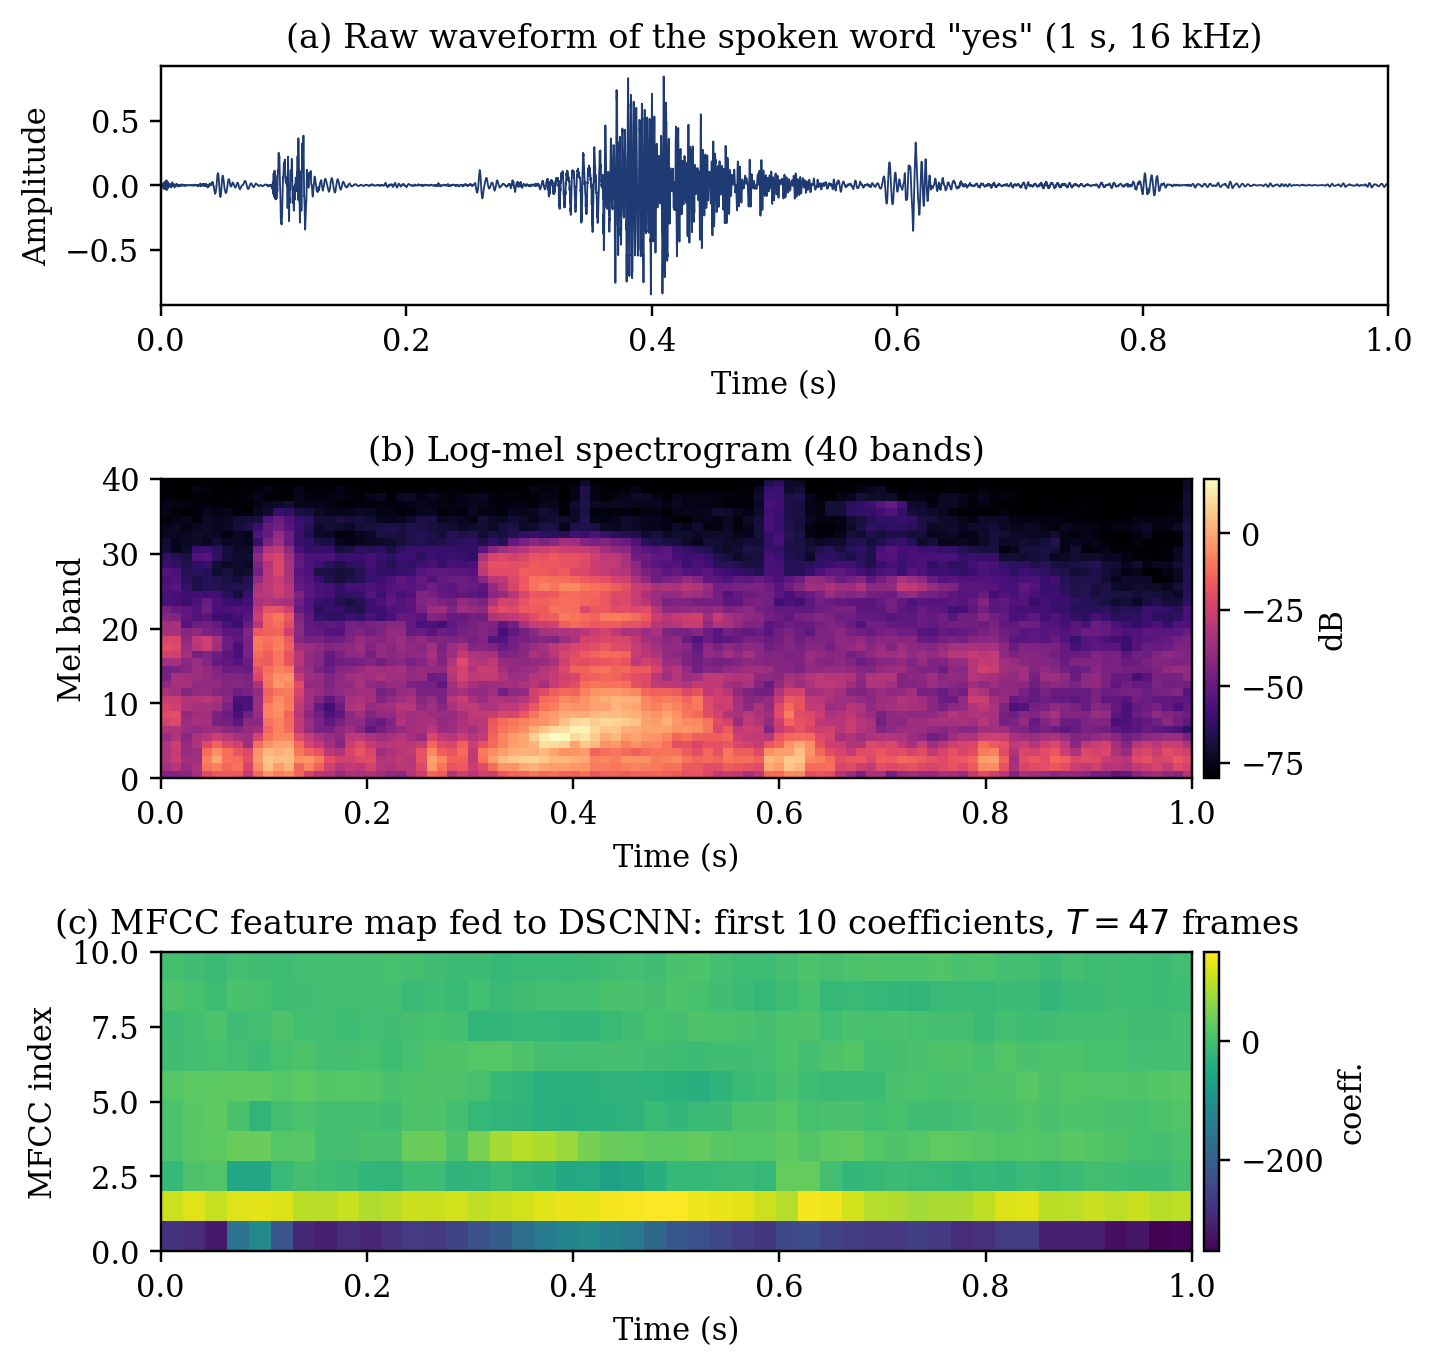
\includegraphics[width=0.92\linewidth]{fig_audio_features.png}
\caption{From sound to features, computed from a real Google Speech Commands
recording of the word ``yes''.
(a) the 1\,s, 16\,kHz raw waveform;
(b) the 40-band log-mel spectrogram (perceptual time--frequency image);
(c) the first 10 MFCC coefficients over $T{=}47$ frames --- the tensor actually
fed to the DSCNN encoder. \emph{Generated from project data with
\code{make\_thesis\_figures.py}.}}
\label{fig:audiofeat}
\end{figure}

\reviewnote{Two new data-illustration figures added below
(\ref{fig:dataexamples}, \ref{fig:melfb}), both generated from real project data,
in the spirit of the sample thesis's dataset-example figures.}

To build intuition for what the model actually sees, \Cref{fig:dataexamples} shows
the log-mel spectrograms of six different command words. Each word has a
characteristic time--frequency signature --- the rising voiced segment of
``yes'', the plosive burst of ``stop'', the nasal onset of ``no'' --- and it is
this structure, not the raw waveform, that the encoder learns to compare.

\begin{figure}[t]
\centering
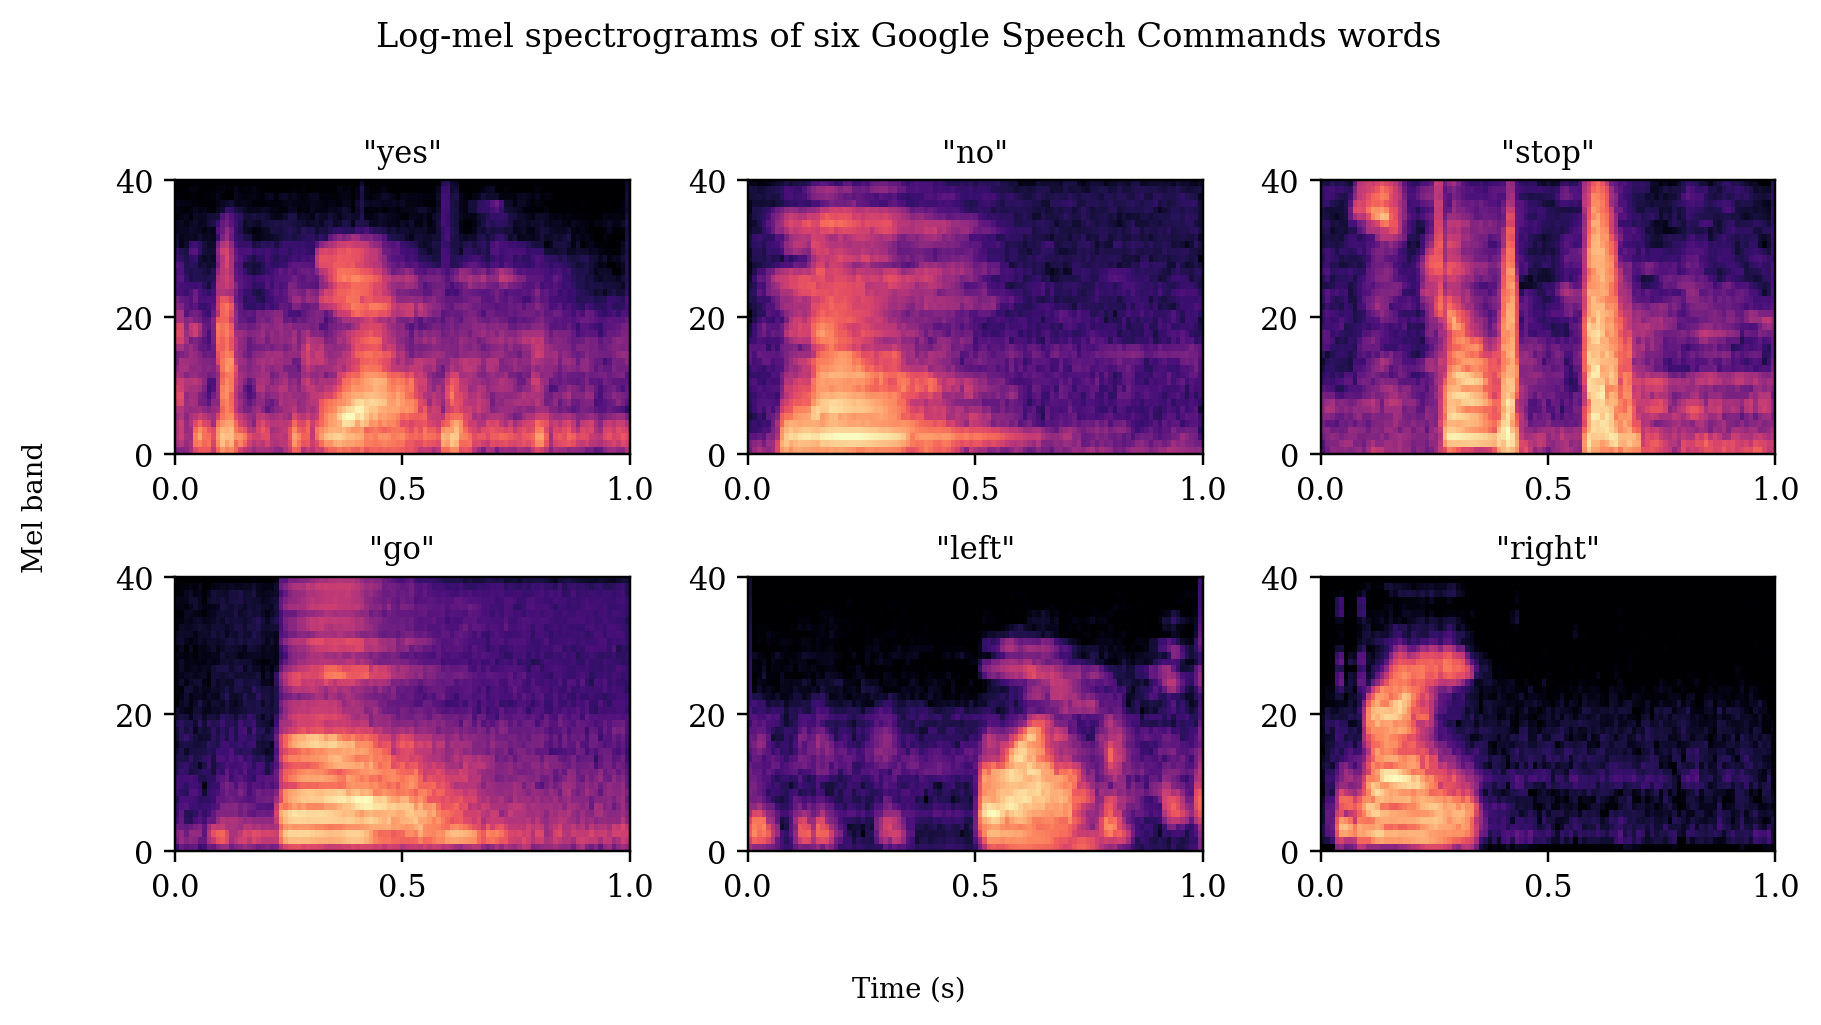
\includegraphics[width=0.95\linewidth]{fig_data_examples.png}
\caption{Log-mel spectrograms of six Google Speech Commands words (real data).
Different words occupy visibly different time--frequency patterns, which is what
makes metric learning in this space effective.}
\label{fig:dataexamples}
\end{figure}

\Cref{fig:melfb} makes the mel front-end concrete: (a) the 40 overlapping
triangular filters that pool STFT energy --- densely packed at low frequencies and
sparse at high frequencies --- and (b) the Hz-to-mel warping of \Cref{eq:mel}.

\begin{figure}[t]
\centering
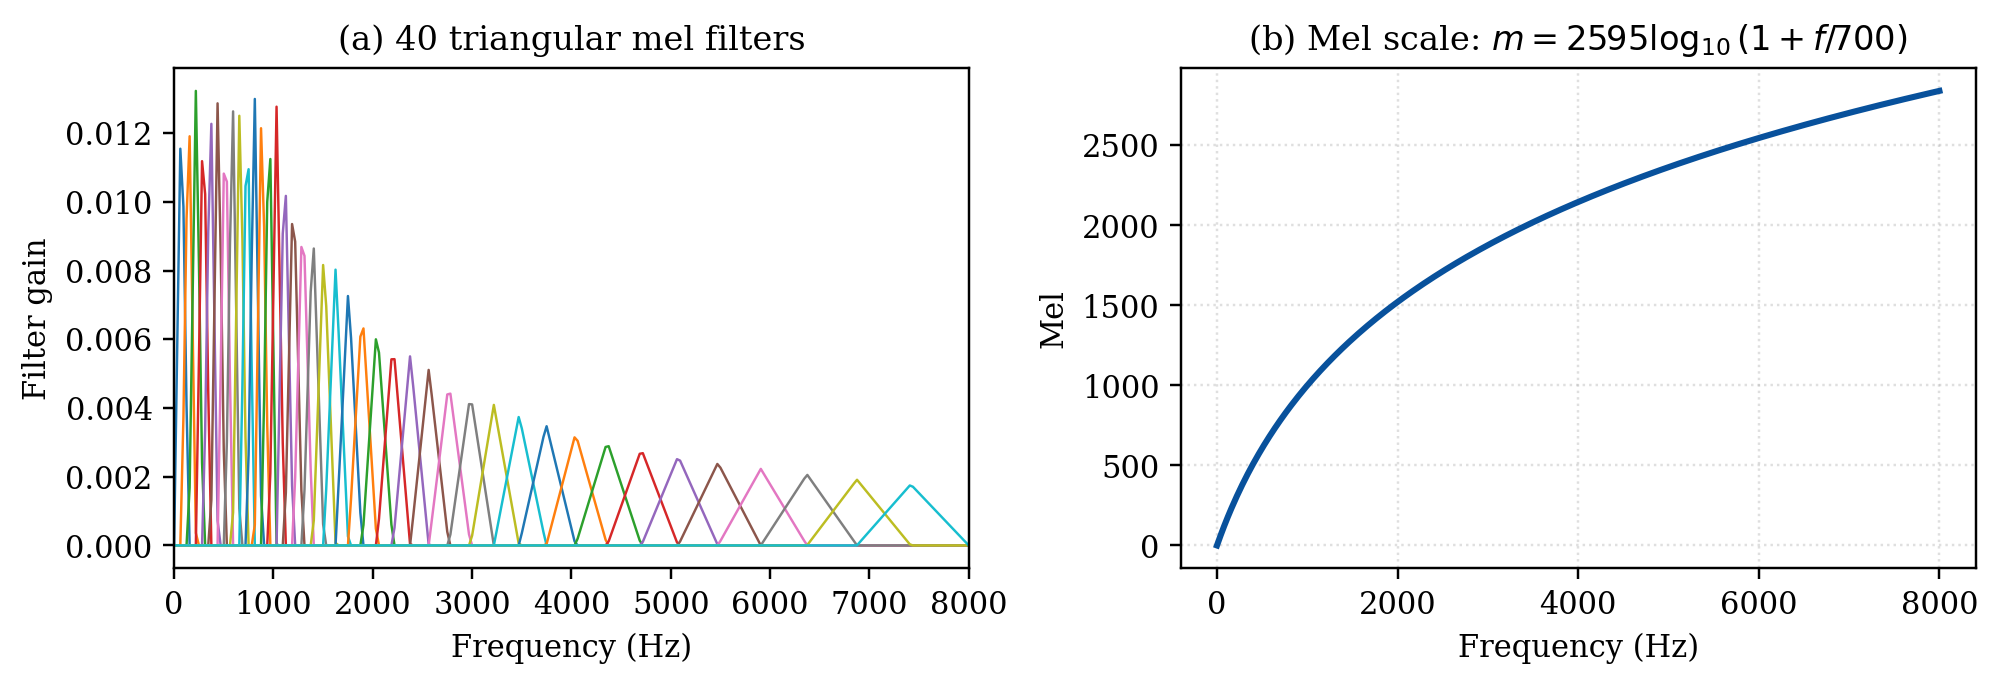
\includegraphics[width=0.95\linewidth]{fig_mel_filterbank.png}
\caption{The mel front-end. (a) the 40-channel triangular mel filterbank used in
this work; (b) the perceptual Hz$\to$mel warping curve. \emph{Generated from the
project's feature code.}}
\label{fig:melfb}
\end{figure}

\section{Keyword spotting: closed-set vs.\ open-set}\label{sec:kws-bg}

Small-footprint KWS was popularized by depthwise-separable convolutional networks
(DS-CNN)~\cite{zhang2017hello} and later refined by broadcasted-residual networks
(BC-ResNet)~\cite{kim2021bcresnet}, both of which trade accuracy against parameter
count for microcontroller deployment. These are \emph{closed-set} classifiers:
they output a probability over a fixed label set and therefore cannot, by design,
abstain on unknown inputs. The open-set requirement --- accepting known keywords
while rejecting everything else --- is what separates a laboratory accuracy number
from a deployable wake-word engine.

\section{Few-shot learning and metric learning}\label{sec:fewshot-bg}

To support \emph{arbitrary} vocabularies we cast KWS as metric learning: the
network learns an embedding space in which utterances of the same word are close
and utterances of different words are far apart. Prototypical
networks~\cite{snell2017prototypical} represent each class by the mean
(``prototype'') of its few support embeddings and classify queries by nearest
prototype; triplet embeddings~\cite{schroff2015facenet} optimize relative
distances directly. The Generalized End-to-End (GE2E) loss~\cite{wan2018ge2e},
originally proposed for speaker verification, builds centroids inside each
training batch exactly as deployment builds prototypes, making it a natural fit
for few-shot KWS. We adopt GE2E as a centroid objective and compare it against
triplet and against angular-margin classification.

\section{Angular-margin classification and open-set rejection}\label{sec:arc-bg}

ArcFace~\cite{deng2019arcface} and its sub-center variant
SCAF~\cite{deng2020subcenter} learn highly discriminative embeddings for face
recognition with thousands of identities by enforcing an angular margin between
classes. A natural question --- which this thesis answers negatively at extreme
scale --- is whether the same machinery transfers to tens of thousands of word
classes. For the open-set decision itself, OpenMax~\cite{bendale2016openmax}
fits Weibull tails to per-class activations, and energy
scores~\cite{liu2020energy} offer a calibration-free alternative; we adapt both
to operate on prototype distances and compare them with a plain nearest-class-mean
threshold. Finally, self-supervised speech models such as
Wav2Vec\,2.0~\cite{baevski2020wav2vec} provide powerful representations; we use a
frozen Wav2Vec\,2.0 only as a distillation \emph{teacher}, keeping the deployed
student tiny.

%==============================================================================
\chapter{Proposed Method}\label{ch:method}
\reviewnote{Chapter~3 collects \emph{what you did and how you measured it}, with
no results (results are in Chapter~4), exactly as you requested. Your provided
blocks --- ``Datasets and Training Protocol'', ``System Architecture'' and the
methodology part of ``Evaluation'' --- are reproduced \textbf{verbatim} below;
text shown \textcolor{addcolor}{in dark blue with a ``+ added'' margin tag} is
material I added, and the pipeline diagram, the experimental-design section
(\ref{sec:expdesign}), and the deployment/streaming section (\ref{sec:deploy})
are new additions noted with their own banners.}

\NEW{At a high level (\Cref{fig:pipeline}) the method has two phases that share a
single, frozen encoder. In the \emph{training phase} the encoder is optimized
once on MSWC with a metric objective. In the \emph{deployment phase} the user
enrolls a few examples per keyword to form prototypes, and queries are recognized
by nearest-prototype distance with an explicit open-set threshold --- the encoder
is never retrained.}

\begin{figure}[t]
\centering
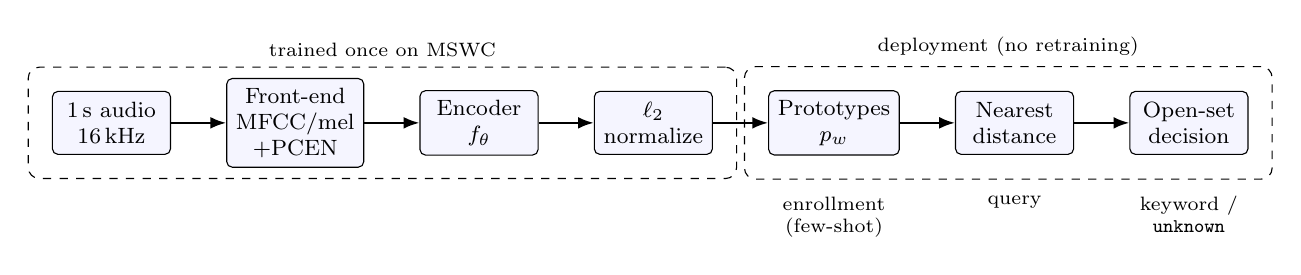
\begin{tikzpicture}[
  node distance=5mm and 7mm,
  box/.style={draw,rounded corners=2pt,align=center,minimum height=8mm,
              minimum width=15mm,font=\footnotesize,fill=blue!4},
  arr/.style={-{Latex[length=2mm]},thick},
  small/.style={font=\scriptsize,align=center}]
\node[box] (wav) {1\,s audio\\16\,kHz};
\node[box,right=of wav] (feat) {Front-end\\MFCC/mel\\$+$PCEN};
\node[box,right=of feat] (enc) {Encoder\\$f_\theta$};
\node[box,right=of enc] (norm) {$\ell_2$\\normalize};
\node[box,right=of norm] (proto) {Prototypes\\$p_w$};
\node[box,right=of proto] (dist) {Nearest\\distance};
\node[box,right=of dist] (dec) {Open-set\\decision};
\draw[arr](wav)--(feat);\draw[arr](feat)--(enc);\draw[arr](enc)--(norm);
\draw[arr](norm)--(proto);\draw[arr](proto)--(dist);\draw[arr](dist)--(dec);
\node[small,below=4mm of proto]{enrollment\\(few-shot)};
\node[small,below=4mm of dist]{query};
\node[small,below=4mm of dec]{keyword /\\\texttt{unknown}};
\begin{scope}[on background layer]
\node[draw,dashed,rounded corners,fit=(wav)(norm),inner sep=3mm,
      label={[font=\scriptsize]above:trained once on MSWC}]{};
\node[draw,dashed,rounded corners,fit=(proto)(dec),inner sep=3mm,
      label={[font=\scriptsize]above:deployment (no retraining)}]{};
\end{scope}
\end{tikzpicture}
\caption{\NEW{End-to-end few-shot open-set KWS pipeline. The encoder is trained
once; at deployment, user keywords become prototypes and queries are classified
by nearest-prototype distance with an open-set threshold.}}
\label{fig:pipeline}
\end{figure}

\section{Problem formulation}\label{sec:formulation}
\reviewnote{Short formalization added so the equations referenced later
(Eq.~\ref{eq:proto}, \ref{eq:score}) are defined.}

Let $f_\theta:\R^{T\times F}\!\to\!\R^{d}$ be an encoder mapping a one-second
representation to a unit-norm embedding. The prototype of a keyword $w$ is the
mean of its $k$ support embeddings,
\begin{equation}
p_w \;=\; \frac{1}{k}\sum_{i=1}^{k} f_\theta\!\big(x^{(w)}_i\big).
\label{eq:proto}
\end{equation}
A query $x$ is assigned to the nearest prototype, with open-set score equal to the
negated minimum distance,
\begin{equation}
\hat w(x)=\arg\min_{w} d\!\big(f_\theta(x),p_w\big),\qquad
s(x)=-\!\min_{w} d\!\big(f_\theta(x),p_w\big),
\label{eq:score}
\end{equation}
and accepted as $\hat w(x)$ iff $s(x)\ge\tau$, otherwise labelled \texttt{unknown}.

\reviewnote{New figure (\ref{fig:embedding}) added: a real t-SNE projection of the
trained model's embedding space, produced by running the best local checkpoint on
GSC. It is the most direct visualization of why the method works and is the
analogue of the sample thesis's ``pipeline output'' figure.}

\Cref{fig:embedding} visualizes the learned space directly. Running the best
trained encoder on real GSC recordings and projecting the embeddings to two
dimensions, each known command forms a tight, well-separated cluster around its
prototype (stars), while out-of-vocabulary words (grey crosses) fall in the gaps
between clusters --- exactly the geometry that makes nearest-prototype matching
with distance thresholding work for open-set rejection.

\begin{figure}[t]
\centering
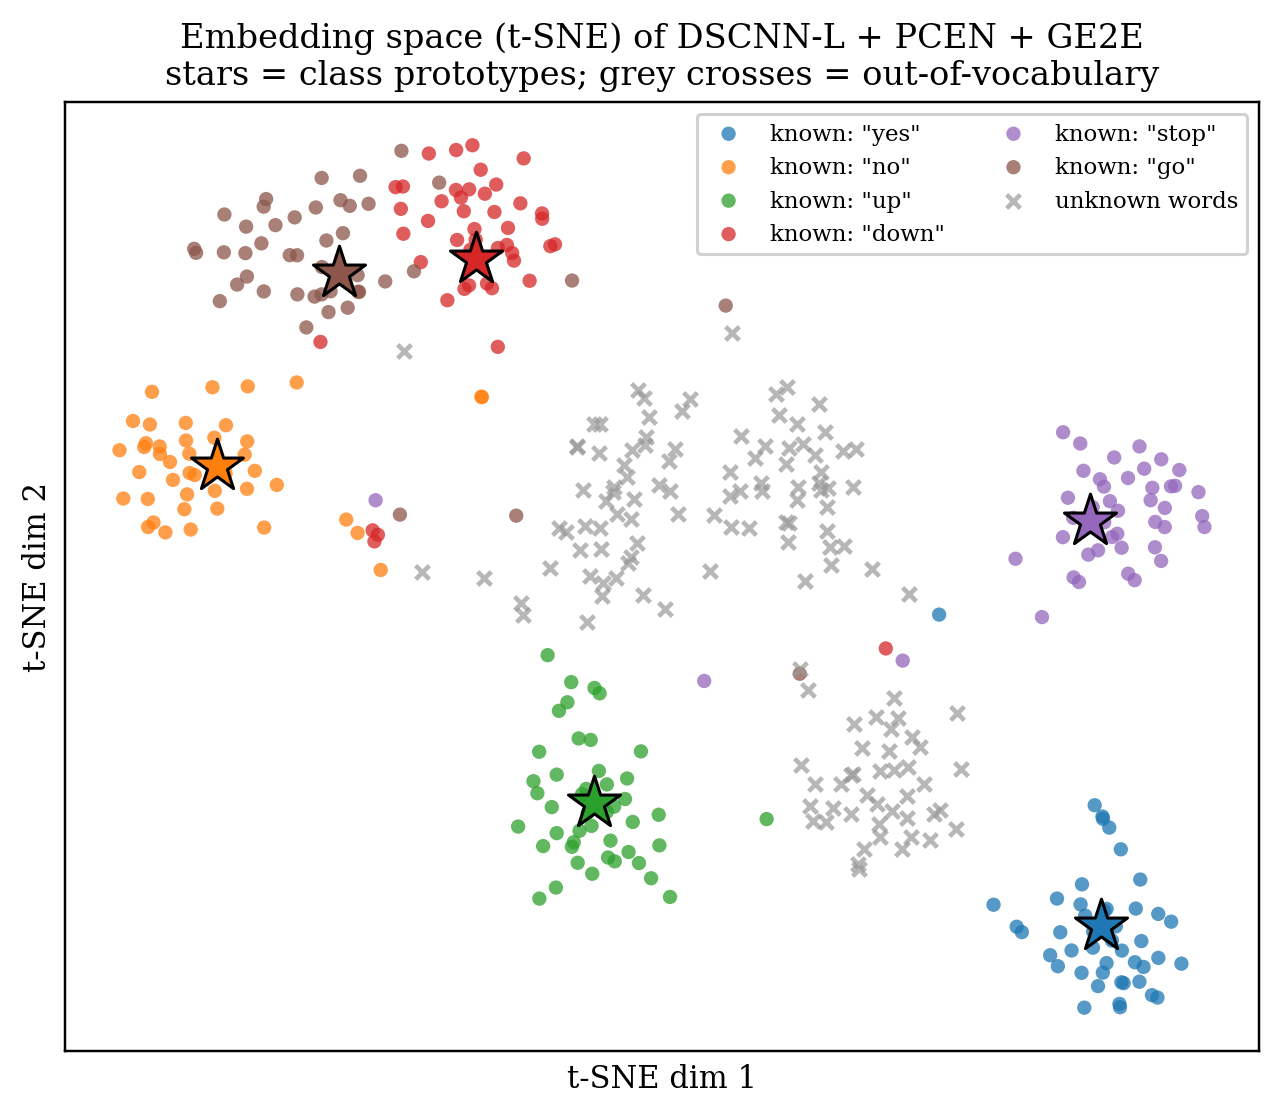
\includegraphics[width=0.86\linewidth]{fig_embedding_space.png}
\caption{\NEW{t-SNE projection of embeddings from the trained DSCNN-L\,+\,PCEN\,+\,GE2E
model on real GSC audio. Coloured points are six known commands, stars are their
prototypes, grey crosses are out-of-vocabulary words. Generated with
\code{make\_inference\_figures.py} from the local checkpoint.}}
\label{fig:embedding}
\end{figure}

\section{Datasets and Training Protocol}\label{sec:data}

\textbf{Training corpus (MSWC English):} We train on the English subset of the
Multilingual Spoken Words Corpus, which after filtering for $\ge$ minimum clips
contains 37,387 training words (and 763 validation words), drawn from a metadata
pool of $\sim$38,150 words and $\sim$6.6\,M clips. To study scale we form caps of
$\{20, 50, 220, 620\}$ clips per word --- roughly $\{0.53, 0.94, 2.05, 2.99\}$\,M
training clips --- and two reduced regimes: a Top-500 legacy split (450 train / 50
val words, evaluation on words ranked 501+ with $\ge 1000$ utterances) and an
MLCommons micro-set (31 keywords) used only for pipeline validation and
architecture screening. \NEW{The three vocabulary regimes span more than three
orders of magnitude (\Cref{fig:vocabscale}); this range is what makes the
scale effects in \Cref{ch:results} observable.}

\begin{figure}[t]
\centering
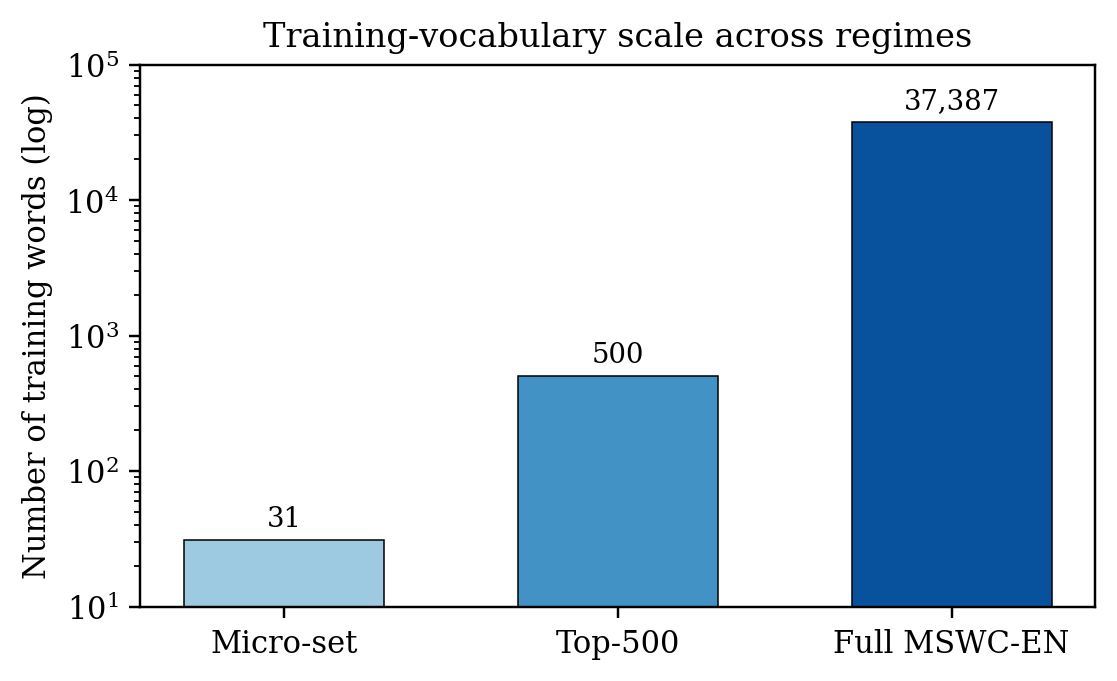
\includegraphics[width=0.72\linewidth]{fig_vocab_scale.png}
\caption{\NEW{Training-vocabulary size for the three regimes (log scale). The
micro-set is used only for screening; full MSWC English is the headline regime.}}
\label{fig:vocabscale}
\end{figure}

\textbf{Episodic sampling and augmentation:} Episodes draw 30 classes $\times$ 20
utterances (only classes with $\ge 20$ clips are eligible). Online augmentation
mixes DEMAND background noise (probability 0.5, SNR sampled in $[0, 10]$\,dB) and
applies SpecAugment (one frequency mask of width 6, one time mask of width 8);
gain perturbation ($\pm6$\,dB) and time-shift ($\le 100$\,ms) are applied with
probability 0.5. \NEW{\Cref{fig:augment} illustrates these augmentations on a real
recording: additive background noise at 5\,dB SNR fills the quiet regions, and the
SpecAugment frequency/time masks (black bands) force the encoder not to rely on any
single band or instant.}

\begin{figure}[t]
\centering
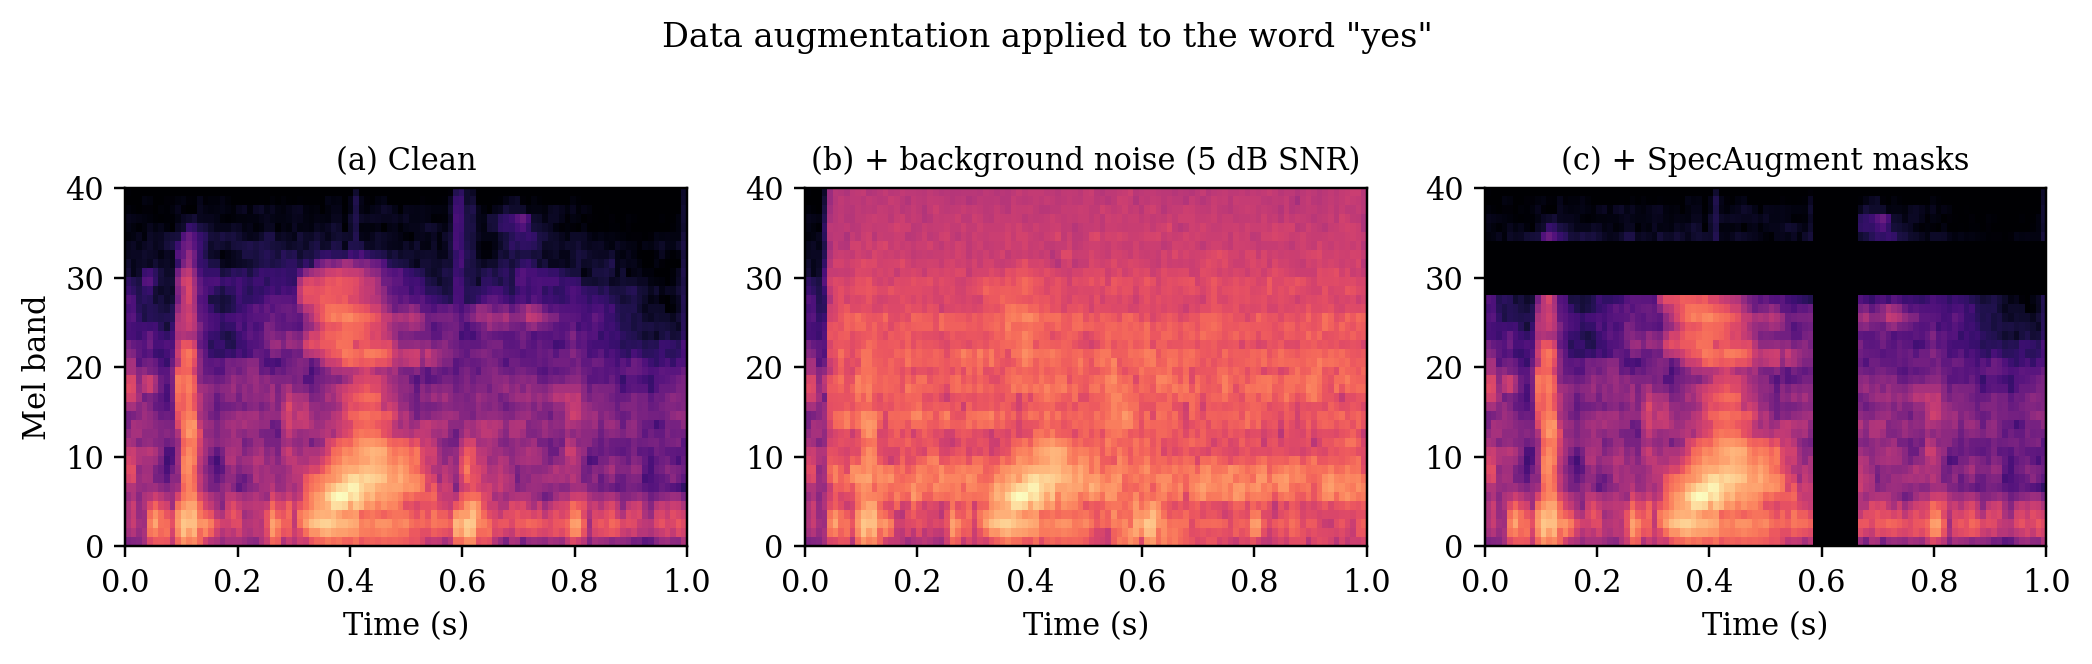
\includegraphics[width=0.98\linewidth]{fig_augmentation.png}
\caption{\NEW{Training-time augmentation on the word ``yes'' (real data):
(a) clean log-mel; (b) $+$ real background noise at 5\,dB SNR; (c) $+$ SpecAugment
frequency and time masks.}}
\label{fig:augment}
\end{figure}

\textbf{Evaluation corpus (GSC v2):} We evaluate cross-corpus on Google Speech
Commands v2. Enrollment (support) samples are drawn from the official
\code{validation\_list.txt}; query samples from \code{testing\_list.txt}
(``test'') or the remaining files (``dev''), preventing leakage. A synthetic
\code{\_silence\_} class is generated from random one-second crops of
\code{\_background\_noise\_}, with disjoint crops for support and query.

\textbf{EdgeSpot-exact protocol:} The headline protocol partitions GSC's 35 words
into 11 positive classes --- the ten command words \{yes, no, up, down, left,
right, on, off, stop, go\} plus \code{\_silence\_} --- and 25 negative (unknown)
spoken words. Each run enrolls $k{=}10$ shots per positive word, computes
prototypes, and scores up to 50 query samples per word (a fixed-seed subsample).
We report the mean$\pm$std over 100 randomized runs; randomness comes from
enrollment-shot selection (the known/unknown vocabulary itself is fixed across
runs). ``test100'' denotes 100 runs on the test split, ``dev30'' denotes 30 runs
on the dev split.

\section{System Architecture}\label{sec:arch}

\subsection{Feature front-ends}\label{sec:frontends}

All audio is mono, 16\,kHz, and trimmed/zero-padded to exactly one second
(16,000 samples). We support two spectral parameterizations, summarized in
\Cref{tab:features}.

\begin{table}[t]
\centering
\caption{Feature front-end configurations.}
\label{tab:features}
\begin{tabular}{lcc}
\toprule
 & \textbf{MFCC} & \textbf{Log-mel} \\
\midrule
Sample rate     & \multicolumn{2}{c}{16\,kHz, mono, 1\,s} \\
FFT size        & 1024  & 512  \\
Window / hop    & 40/20\,ms & 25/10\,ms \\
\code{center}   & \code{False} & \code{True} \\
Mel bands       & 40 & 40 \\
Output coeffs.  & 10 (first DCT) & 40 (mel) \\
Tensor shape    & $(1,47,10)$ & $(1,40,101)$ \\
Trainable PCEN  & optional & optional \\
\bottomrule
\end{tabular}
\end{table}

\textbf{MFCC (DSCNN front-end):} We compute 40 Mel-frequency cepstral
coefficients with a 1024-point FFT, 640-sample (40\,ms) Hann window, 320-sample
(20\,ms) hop, and \code{center=False}; the Mel filterbank uses Slaney scale and
Slaney area normalization, and the log is taken as $10\log_{10}(\cdot)$ followed
by an orthonormal DCT-II. We retain only the first 10 coefficients and transpose
to a tensor of shape $(1,47,10)=(\text{channel}, T_{\text{frames}},
\text{features})$, where $T = 47 = \lfloor(16000-1024)/320\rfloor + 1$.

\textbf{Log-mel (EdgeSpot/BC-ResNet front-end):} We use 40 Mel bands with a
512-point FFT, 400-sample (25\,ms) window, 160-sample (10\,ms) hop and
\code{center=True}, producing $(1,40,101)$. The log compression is delegated to
the PCEN layer.

\textbf{Trainable PCEN:} Per-channel energy normalization~\cite{wang2017trainable}
applies a causal first-order IIR smoother $M_t = (1-s)M_{t-1} + sE_t$ followed by
adaptive gain and dynamic-range compression,
\begin{equation}
\text{PCEN}(E_t)=\Big(\frac{E_t}{(\epsilon+M_t)^{\alpha}}+\delta\Big)^{r}-\delta^{r},
\label{eq:pcen}
\end{equation}
with learnable $\alpha,\delta,r,s$ (initialized to $0.96, 2.0, 0.5, 0.04$;
$\epsilon{=}10^{-6}$). PCEN replaces the static log and adapts to channel
statistics during training.

\subsection{Encoders}\label{sec:encoders}

\textbf{DSCNN-L:} A depthwise-separable CNN built from a size table: an initial
$\text{Conv}(1{\to}276, 10{\times}4, \text{stride } 2{\times}1)$ with
TensorFlow-style asymmetric ``same'' padding, followed by five depthwise separable
blocks (276 channels, $3{\times}3$ kernels; the first block strides $2{\times}2$).
All but the last block use BatchNorm+ReLU; the last block uses an (affine-free)
LayerNorm. A global average pool yields the embedding directly, so the embedding
dimension equals the channel width, $d = 276$ (there is no final linear
projection). DSCNN-L has $\approx 0.413$\,M parameters.

\textbf{EdgeSpot-Full ($\tau{=}4$):} A width-scaled edge encoder operating on the
$(1,40,101)$ mel/PCEN input. A $5{\times}5$ stride-$(2,1)$ stem feeds four stages
of fused-temporal and broadcasted-residual ``lite'' blocks with increasing
temporal dilation $(1,2,4,8)$; a depthwise frequency-collapse block averages over
frequency to a $(C,T)$ sequence; a depthwise positional convolution and a
single-head temporal self-attention block ($d = 64$) model long-range temporal
structure; finally a depthwise temporal head and global pooling produce a
64-dimensional embedding. EdgeSpot-Full $\tau{=}4$ has $\approx 0.131$\,M
parameters, $\sim$3.2$\times$ smaller than DSCNN-L. A lighter EdgeSpot-Lite
variant and a clean BC-ResNet-FS baseline (no attention) are also provided.

\begin{table}[t]
\centering
\caption{Encoder comparison. $\ell_2$-normalization is applied outside the
encoder so all losses and the deployment classifier operate on the hypersphere.}
\label{tab:encoders}
\begin{tabular}{lccc}
\toprule
\textbf{Encoder} & \textbf{Front-end} & \textbf{$d$} & \textbf{Params} \\
\midrule
DSCNN-L              & MFCC / mel($+$PCEN) & 276 & 0.413\,M \\
EdgeSpot-Full $\tau{=}4$ & mel($+$PCEN)    & 64  & 0.131\,M \\
EdgeSpot-Lite       & mel($+$PCEN)        & 64  & $<0.131$\,M \\
BC-ResNet-FS $\tau{=}4$  & mel($+$PCEN)    & 64  & $\sim$0.1\,M \\
\bottomrule
\end{tabular}
\end{table}

\reviewnote{New: two TikZ block diagrams of the encoders (\ref{fig:dscnn},
\ref{fig:edgespot}) --- the analogue of the sample thesis's architecture figures,
but drawn to our exact custom networks (they are not public diagrams), plus an
accuracy-vs-size figure (\ref{fig:tradeoff}) analogous to the sample's model-size
comparison.}

\begin{figure}[t]
\centering
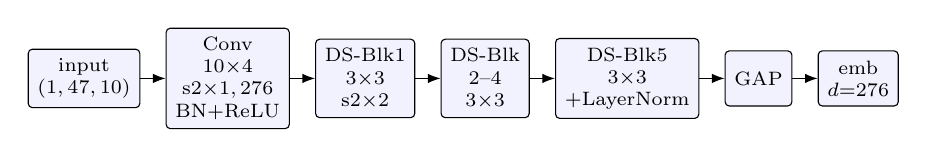
\begin{tikzpicture}[
  font=\scriptsize, node distance=3.2mm,
  b/.style={draw,rounded corners=1.5pt,minimum height=7mm,align=center,fill=blue!5},
  a/.style={-{Latex[length=1.6mm]}}]
\node[b] (in) {input\\$(1,47,10)$};
\node[b,right=of in] (c0) {Conv\\$10{\times}4$\\s$2{\times}1$,\,276\\BN+ReLU};
\node[b,right=of c0] (d1) {DS-Blk1\\$3{\times}3$\\s$2{\times}2$};
\node[b,right=of d1] (d2) {DS-Blk\\2--4\\$3{\times}3$};
\node[b,right=of d2] (d5) {DS-Blk5\\$3{\times}3$\\+LayerNorm};
\node[b,right=of d5] (gap) {GAP};
\node[b,right=of gap] (emb) {emb\\$d{=}276$};
\draw[a](in)--(c0);\draw[a](c0)--(d1);\draw[a](d1)--(d2);\draw[a](d2)--(d5);
\draw[a](d5)--(gap);\draw[a](gap)--(emb);
\end{tikzpicture}
\caption{\NEW{DSCNN-L encoder: depthwise-separable CNN, $\approx$0.41\,M params.
The embedding equals the final channel width (276); no linear projection.}}
\label{fig:dscnn}
\end{figure}

\begin{figure}[t]
\centering
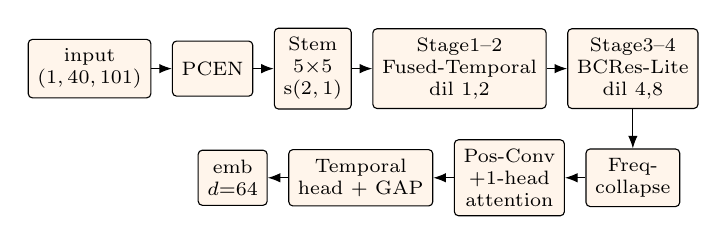
\begin{tikzpicture}[
  font=\scriptsize, node distance=2.6mm,
  b/.style={draw,rounded corners=1.5pt,minimum height=7mm,align=center,fill=orange!8},
  a/.style={-{Latex[length=1.6mm]}}]
\node[b] (in) {input\\$(1,40,101)$};
\node[b,right=of in] (pc) {PCEN};
\node[b,right=of pc] (st) {Stem\\$5{\times}5$\\s$(2,1)$};
\node[b,right=of st] (s12) {Stage1--2\\Fused-Temporal\\dil 1,2};
\node[b,right=of s12] (s34) {Stage3--4\\BCRes-Lite\\dil 4,8};
\node[b,below=5mm of s34] (fc) {Freq-\\collapse};
\node[b,left=of fc] (att) {Pos-Conv\\$+$1-head\\attention};
\node[b,left=of att] (th) {Temporal\\head + GAP};
\node[b,left=of th] (emb) {emb\\$d{=}64$};
\draw[a](in)--(pc);\draw[a](pc)--(st);\draw[a](st)--(s12);\draw[a](s12)--(s34);
\draw[a](s34)--(fc);\draw[a](fc)--(att);\draw[a](att)--(th);\draw[a](th)--(emb);
\end{tikzpicture}
\caption{\NEW{EdgeSpot-Full ($\tau{=}4$) encoder: mel/PCEN front-end, fused-temporal
and broadcasted-residual blocks with growing dilation, frequency collapse, a
single-head temporal self-attention stage, $\approx$0.13\,M params.}}
\label{fig:edgespot}
\end{figure}

\begin{figure}[t]
\centering
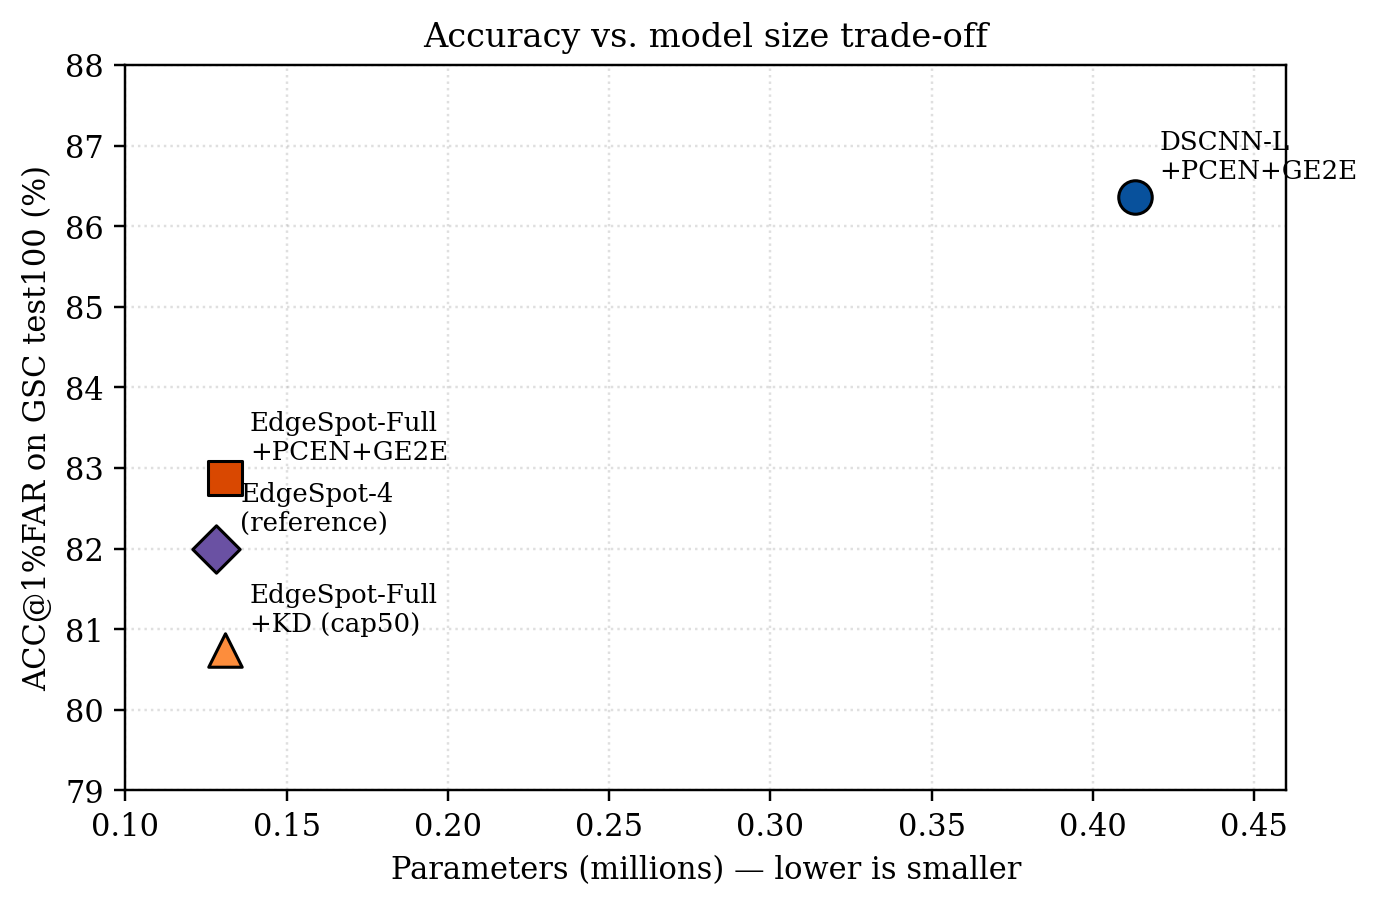
\includegraphics[width=0.78\linewidth]{fig_model_tradeoff.png}
\caption{\NEW{Accuracy vs.\ model size. DSCNN-L leads on accuracy; EdgeSpot-Full
reaches a competitive point at one third the parameters; KD lifts the compact
model further at low data. (Accuracy numbers are detailed in \Cref{ch:results}.)}}
\label{fig:tradeoff}
\end{figure}

\subsection{Metric-learning objectives}\label{sec:losses}

All objectives are trained episodically: each episode samples $n_{\text{cls}}{=}30$
classes with $n_{\text{spp}}{=}20$ utterances each (600 embeddings/episode).

\textbf{Triplet:} Semi-hard triplet loss~\cite{schroff2015facenet} with Euclidean
distance, $\mathcal{L}=\frac{1}{N}\sum\max(0, d(a,p)-d(a,n)+m)$, with
hardest-positive mining and FaceNet semi-hard negative mining.

\textbf{Sub-center ArcFace (SCAF):} An angular-margin softmax with $K{=}3$
sub-centers per class. With normalized weights $W\in\R^{(C\cdot K)\times d}$, the
per-class logit is the max cosine over its sub-centers,
$\cos\theta_c = \max_{j\le K} w_{c,j}^{\top} z$; the additive margin $m{=}0.5$ is
applied to the target class and logits are scaled by $s{=}30$ before
cross-entropy.

\textbf{GE2E (centroid):} Generalized end-to-end loss~\cite{wan2018ge2e} that
mirrors deployment: within an episode each class is split into support/query; the
centroid is the $\ell_2$-normalized support mean and queries are classified by
scaled cosine similarity to all centroids with learnable scale and bias, optimized
by cross-entropy. GE2E directly optimizes the enroll-then-match objective of
\Cref{eq:proto,eq:score}.

\textbf{Cosine knowledge distillation (KD):} We additionally distill from a frozen
Wav2Vec\,2.0-base teacher (hidden layer 16, mean-pooled, projected to $d{=}64$ by
a sub-center-ArcFace-trained head). The distillation loss is a pure
embedding-cosine term,
\begin{equation}
\mathcal{L}_{\text{KD}} = 1 - \frac{1}{N}\sum_i
\cos\!\big(f_\theta(x_i),\, g_{\text{teacher}}(x_i)\big),
\label{eq:kd}
\end{equation}
i.e.\ no temperature/soft-label term. Teacher embeddings are precomputed offline
and looked up by file path during training.

\textbf{Hybrid combinations:} We form weighted sums, e.g.\ \code{scaf\_ge2e},
\code{kd\_ge2e}, \code{kd\_scaf}, \code{kd\_scaf\_ge2e}. A crucial implementation
detail (and a key empirical finding, \Cref{ch:results}) is the SCAF weight: under
KD it is set to $5\times10^{-5}$ while GE2E/KD weights are 1.0. The very small
SCAF weight prevents the high-magnitude angular-margin classification loss from
dominating the centroid/cosine terms.

\NEW{\textbf{Optimization.} Unless noted, training uses Adam (learning rate
$10^{-3}$, weight decay $10^{-4}$), gradient clipping at $5.0$, a
cosine-annealing-with-warm-restarts schedule ($T_0{=}10$, $T_{\text{mult}}{=}2$,
$\eta_{\min}{=}10^{-5}$), and a fixed seed (42) with cuDNN determinism for
reproducibility. Per-experiment epoch/episode budgets are stated in
\Cref{ch:results}.}

\section{Open-set rejection heads}\label{sec:openset}
\reviewnote{Subsection added to document the four rejection heads you implemented
(your draft mentioned them only in the abstract's contribution list).}

All heads share the prototype interface and differ only in the rejection score;
the predicted keyword is always the argmin-distance class (\Cref{eq:score}).
(i) \textbf{Nearest-class-mean (NCM, ``Direct $\ell_2$'')} --- our default ---
rejects when the minimum prototype distance exceeds a threshold, using raw
distances with no probability normalization.
(ii) \textbf{OpenMax}~\cite{bendale2016openmax} fits a Weibull tail to
support-to-prototype distances and uses $1-\mathrm{CDF}$ as the membership score.
(iii) \textbf{Energy}~\cite{liu2020energy} treats $-d_i$ as logits and uses the
free energy $E(x)=T\log\sum_i\exp(-d_i/T)$ as the acceptance score.
(iv) \textbf{Calibrated} thresholds ($\mu+2\sigma$ of support distances) drive
per-word confusion analysis.

\section{Evaluation methodology}\label{sec:eval}

We treat the open-set problem as a binary keyword-vs-non-keyword detection
augmented by a multiclass identity track, and build all metrics on the ROC.
\begin{itemize}[leftmargin=1.3em,itemsep=1pt]
\item \textbf{AUC:} area under the ROC of the open-set scores (\Cref{eq:score});
threshold-free.
\item \textbf{EER:} equal-error rate, the operating point minimizing
$|\far-\frr|$, reported as $(\far+\frr)/2$.
\item \textbf{FRR@FAR:} false-reject rate at the largest threshold whose
false-accept rate does not exceed the target (1\% or 5\%).
\item \textbf{Open-set ACC@FAR:} the headline accuracy. A known query is correct
iff it is accepted ($s\ge\tau_{\far}$) and the argmin label is correct; an unknown
query is correct iff it is rejected. Reported at $\far\in\{1\%, 5\%\}$.
\item \textbf{Keyword ACC:} closed-set nearest-prototype accuracy over known
queries only (ignores rejection).
\item \textbf{F1:} binary keyword-vs-unknown F1 at the EER threshold.
\end{itemize}

\textbf{Interpretation caveat.} AUC and EER are threshold-free, whereas ACC@FAR
and FRR@FAR use a threshold derived from the evaluation ROC (an oracle operating
point), not transferred from a held-out calibration split. We therefore treat
ACC@FAR as a comparison metric across systems under matched conditions, and report
AUC/EER/F1 jointly so that degenerate operating points are visible. A system that
rejects nearly everything can score a high open-set ACC against many negatives
while missing all positives; such cases are exposed by $\frr\to100\%$ and
$\text{F1}\to0$.

\section{Experimental design: what we measure}\label{sec:expdesign}
\reviewnote{New section. It states the four questions the experiments answer
(without giving results --- results are Chapter~4), so Chapter~4 has a clear
narrative to report against.}

The experiments are organized around four questions:
\begin{description}[leftmargin=1.6em,itemsep=2pt]
\item[\textbf{Q1 --- Which design axis matters?}] We train all
$2{\times}2{\times}4 = 16$ combinations of \{DSCNN-L, EdgeSpot-Full\} $\times$
\{MFCC, PCEN\} $\times$ \{Triplet, SCAF, GE2E, SCAF$+$GE2E\} on full-vocabulary
MSWC and isolate each axis with \emph{paired deltas} (changing one factor while
holding the others fixed).
\item[\textbf{Q2 --- How does performance scale?}] Fixing the best front-end and
loss, we sweep the per-word cap $\{20,50,220,620\}$ and grow the vocabulary from
31 to 37,387 words, watching for both saturation and failure.
\item[\textbf{Q3 --- Can distillation replace data?}] We compare GE2E against the
cosine-KD objective at matched data caps.
\item[\textbf{Q4 --- What is the best deployable system?}] We consolidate the
strongest configurations per data regime and identify the best overall and best
compact operating points.
\end{description}

\section{Deployment: streaming and demonstrator}\label{sec:deploy}
\reviewnote{New section documenting the on-device/streaming pipeline and the web
demo you built. Two items here need figures you should export from Colab/your
machine --- see the red boxes.}

Beyond the core encoder, the system includes a CPU streaming pipeline and an
offline web demonstrator. Streaming performs sliding-window detection (1\,s
window, 0.5\,s stride) gated by Silero Voice Activity Detection (VAD): only
windows that VAD marks as speech are embedded and matched, reducing computation
and false activations on silence. A backend-agnostic decision \emph{state
machine} (\Cref{alg:sm}) stabilizes raw candidates into clean events using
majority-vote smoothing over a short window, a top-2 margin check, and a cooldown
to suppress duplicate firings. Optional modules --- a spectral-gating/SpeechBrain
denoiser and an ECAPA-TDNN speaker-verification gate --- follow the same
fail-open, runtime-toggle pattern. The pipeline is designed to a per-component CPU
budget (VAD $<5$\,ms/chunk, MFCC $<5$\,ms, encoder $<10$\,ms, classifier
$<1$\,ms; core $<21$\,ms; $<71$\,ms with all enhancements); a measured on-device
benchmark is left to future work.

\begin{algorithm}[t]
\caption{Streaming decision state machine (smoothing $+$ cooldown).}
\label{alg:sm}
\footnotesize
\begin{algorithmic}[1]
\Require window $W$, votes $V$, margin $m_{\min}$, cooldown $C$
\State buffer $\gets$ deque(maxlen $=W$);\ $t_{\text{last}}\gets-\infty$
\For{each candidate $c$ with span $[t_s,t_e]$}
  \If{$t_s - t_{\text{last}} < C$} \State emit \textsc{cooldown};\ \textbf{continue} \EndIf
  \If{$\lnot c.\text{detected}$ \textbf{or} $c.\text{kw}{=}$\texttt{unknown}
       \textbf{or} $c.\text{margin}<m_{\min}$}
     \State clear buffer; emit \textsc{rejected};\ \textbf{continue}
  \EndIf
  \State push $c$;\ $k^\star\gets$ majority keyword in buffer
  \If{votes$(k^\star)\ge V$}
     \State $a\gets\arg\max_{\text{conf}}\{c\in\text{buffer}: c.\text{kw}{=}k^\star\}$
     \State $t_{\text{last}}\gets a.t_e$; clear buffer; emit \textsc{detected}$(k^\star)$
  \Else\ \State emit \textsc{scoring} \EndIf
\EndFor
\end{algorithmic}
\end{algorithm}

\colabfig{A screenshot of the offline web demonstrator (model switcher +
long-audio timing view). Export from your local demo at 1280$\times$720 and save
as \code{assets/demo\_ui.png}; then replace this box with
\code{\textbackslash includegraphics}.}

%==============================================================================
\chapter{Results and Analysis}\label{ch:results}
\reviewnote{This entire chapter is new (your draft stopped before results). It
reports and analyzes the measured numbers and references the result figures in
\code{assets/}. Two optional figures (training/collapse curves) are marked as
Colab exports.}

All numbers are mean$\pm$std over the EdgeSpot-exact 10-shot protocol (100 runs on
GSC test, denoted test100). Higher is better for ACC/AUC/F1/Keyword-ACC; lower is
better for EER/FRR.

\section{Training dynamics}\label{sec:res-train}
\reviewnote{New section. \Cref{fig:traincurves} is plotted from \emph{real local
TensorBoard logs} (no re-training needed), and is the analogue of the sample
thesis's ``Training and Validation Loss'' figures.}

\Cref{fig:traincurves} shows the real training trajectory of the Microset anchor
model (EdgeSpot-Full + SCAF+GE2E), read directly from the saved TensorBoard logs.
The SCAF+GE2E loss decreases smoothly from $\sim$15.5 to $\sim$1.3, the validation
AUC rises to and stabilizes near $98\%$, and the GSC-dev open-set accuracy plateaus
around $85\%$ --- a healthy, non-overfitting trajectory. (The contrasting
\emph{collapse} behaviour at full $37$k-class vocabulary is discussed in
\Cref{sec:res-q2}.)

\begin{figure}[t]
\centering
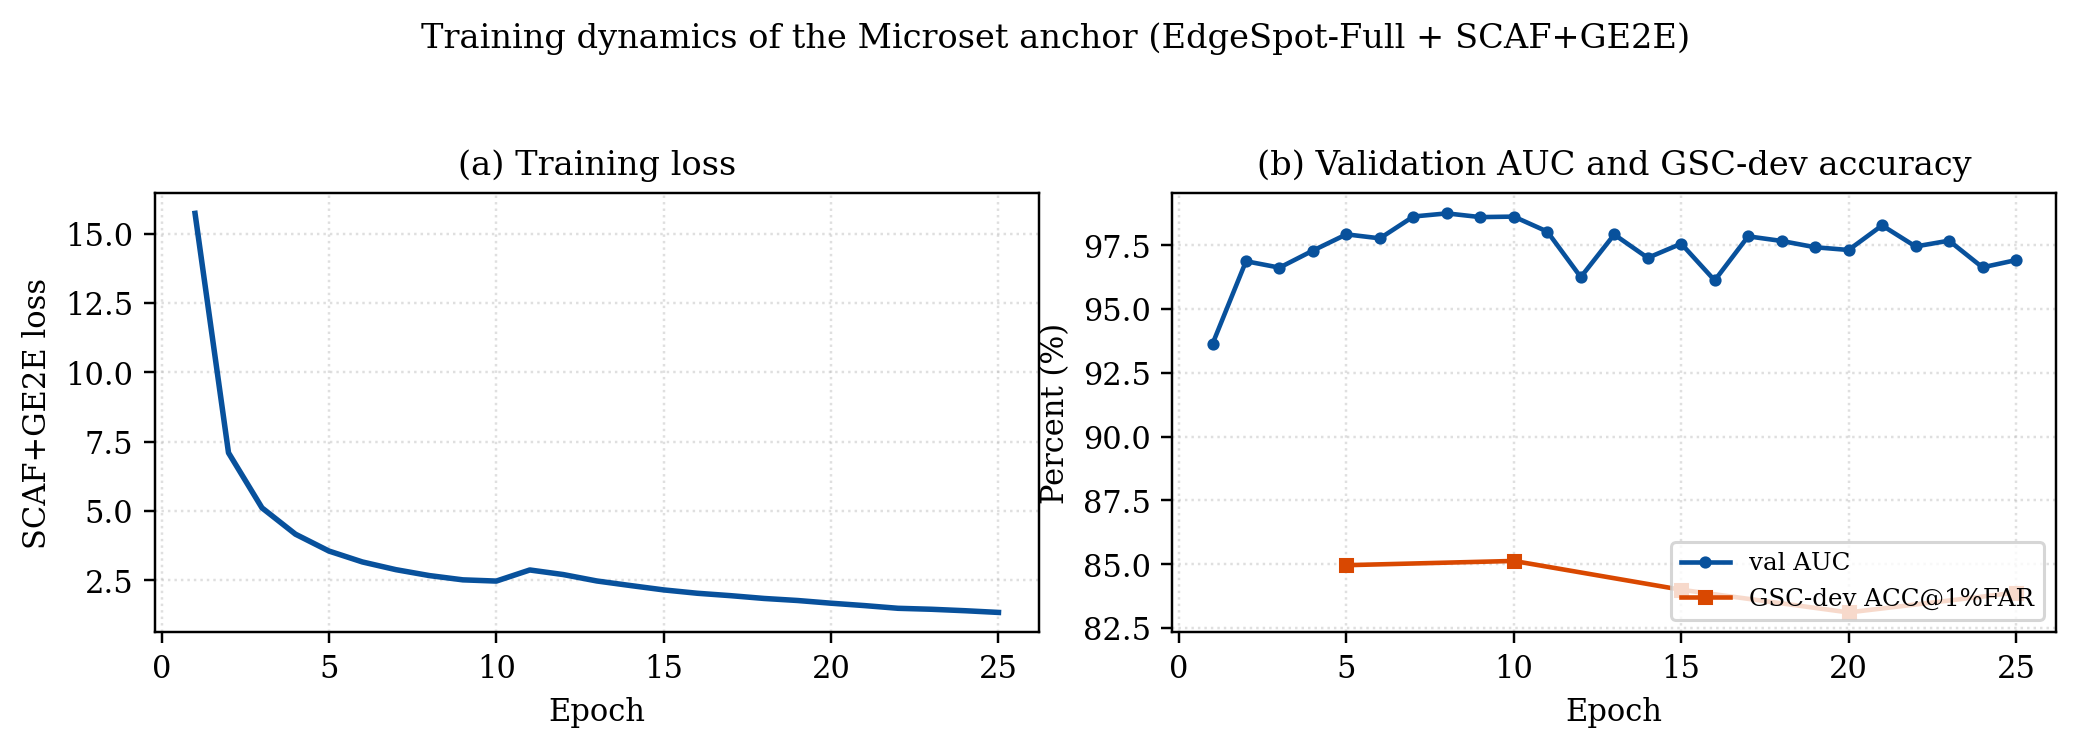
\includegraphics[width=0.98\linewidth]{fig_training_curves.png}
\caption{\NEW{Real training dynamics of the Microset anchor (EdgeSpot-Full +
SCAF+GE2E), from local TensorBoard logs: (a) training loss; (b) validation AUC and
GSC-dev ACC@1\%FAR over epochs. Generated with \code{make\_training\_curves.py}.}}
\label{fig:traincurves}
\end{figure}

\section{Q1: Which design axis matters}\label{sec:res-q1}

\Cref{tab:matrix} reports the full 16-configuration screen on full-vocabulary
MSWC (cap-620), and \Cref{fig:ranked} ranks the configurations visually. Two
findings are immediate: PCEN-based pipelines occupy the top of the ranking, and
the centroid GE2E loss is the best objective for every backbone. The
classification objective SCAF (and the SCAF$+$GE2E hybrid at full weight)
\emph{collapses} at this scale --- a phenomenon analyzed in \Cref{sec:res-q2}.

\begin{table}[t]
\centering
\caption{Full 16-configuration screen on full-vocabulary MSWC (cap-620),
GSC test100 @ 1\% FAR. ``coll.'' marks degenerate collapse
($\auc{=}50$, $\text{F1}{=}0$, $\frr{=}100\%$). Best in bold.}
\label{tab:matrix}
\small
\setlength{\tabcolsep}{4pt}
\begin{tabular}{lll r r r r}
\toprule
\textbf{Enc.} & \textbf{Feat.} & \textbf{Loss} &
\acc$_{1\%}$ & \auc & \eer & F1\\
\midrule
DSCNN & MFCC & Triplet     & 71.52 & 75.55 & 31.41 & 57.17 \\
DSCNN & MFCC & SCAF        & 70.08 & 55.04 & 46.41 & 41.38 \\
DSCNN & MFCC & GE2E        & 77.08 & 86.46 & 21.95 & 68.50 \\
DSCNN & MFCC & SCAF+GE2E   & 69.04 & 47.78 & 52.15 & 35.93 \\
DSCNN & PCEN & Triplet     & 79.98 & 90.65 & 17.57 & 74.14 \\
DSCNN & PCEN & SCAF        & 69.44 & 50.00 & 50.00 & coll. \\
\rowcolor{blue!7}
DSCNN & PCEN & GE2E        & \best{82.34} & \best{92.42} & \best{14.89} & \best{77.75} \\
DSCNN & PCEN & SCAF+GE2E   & 69.44 & 50.00 & 50.00 & coll. \\
Edge  & MFCC & Triplet     & 69.63 & 52.84 & 48.05 & 39.79 \\
Edge  & MFCC & SCAF        & 69.44 & 50.00 & 50.00 & coll. \\
Edge  & MFCC & GE2E        & 70.76 & 65.30 & 39.05 & 48.82 \\
Edge  & MFCC & SCAF+GE2E   & 69.67 & 50.88 & 50.39 & 37.57 \\
Edge  & PCEN & Triplet     & 79.58 & 89.85 & 18.22 & 73.29 \\
Edge  & PCEN & SCAF        & 69.44 & 50.00 & 50.00 & coll. \\
\rowcolor{blue!7}
Edge  & PCEN & GE2E        & \best{79.98} & 87.23 & 20.23 & 70.68 \\
Edge  & PCEN & SCAF+GE2E   & 69.44 & 50.00 & 50.00 & coll. \\
\bottomrule
\end{tabular}
\end{table}

\begin{figure}[t]
\centering
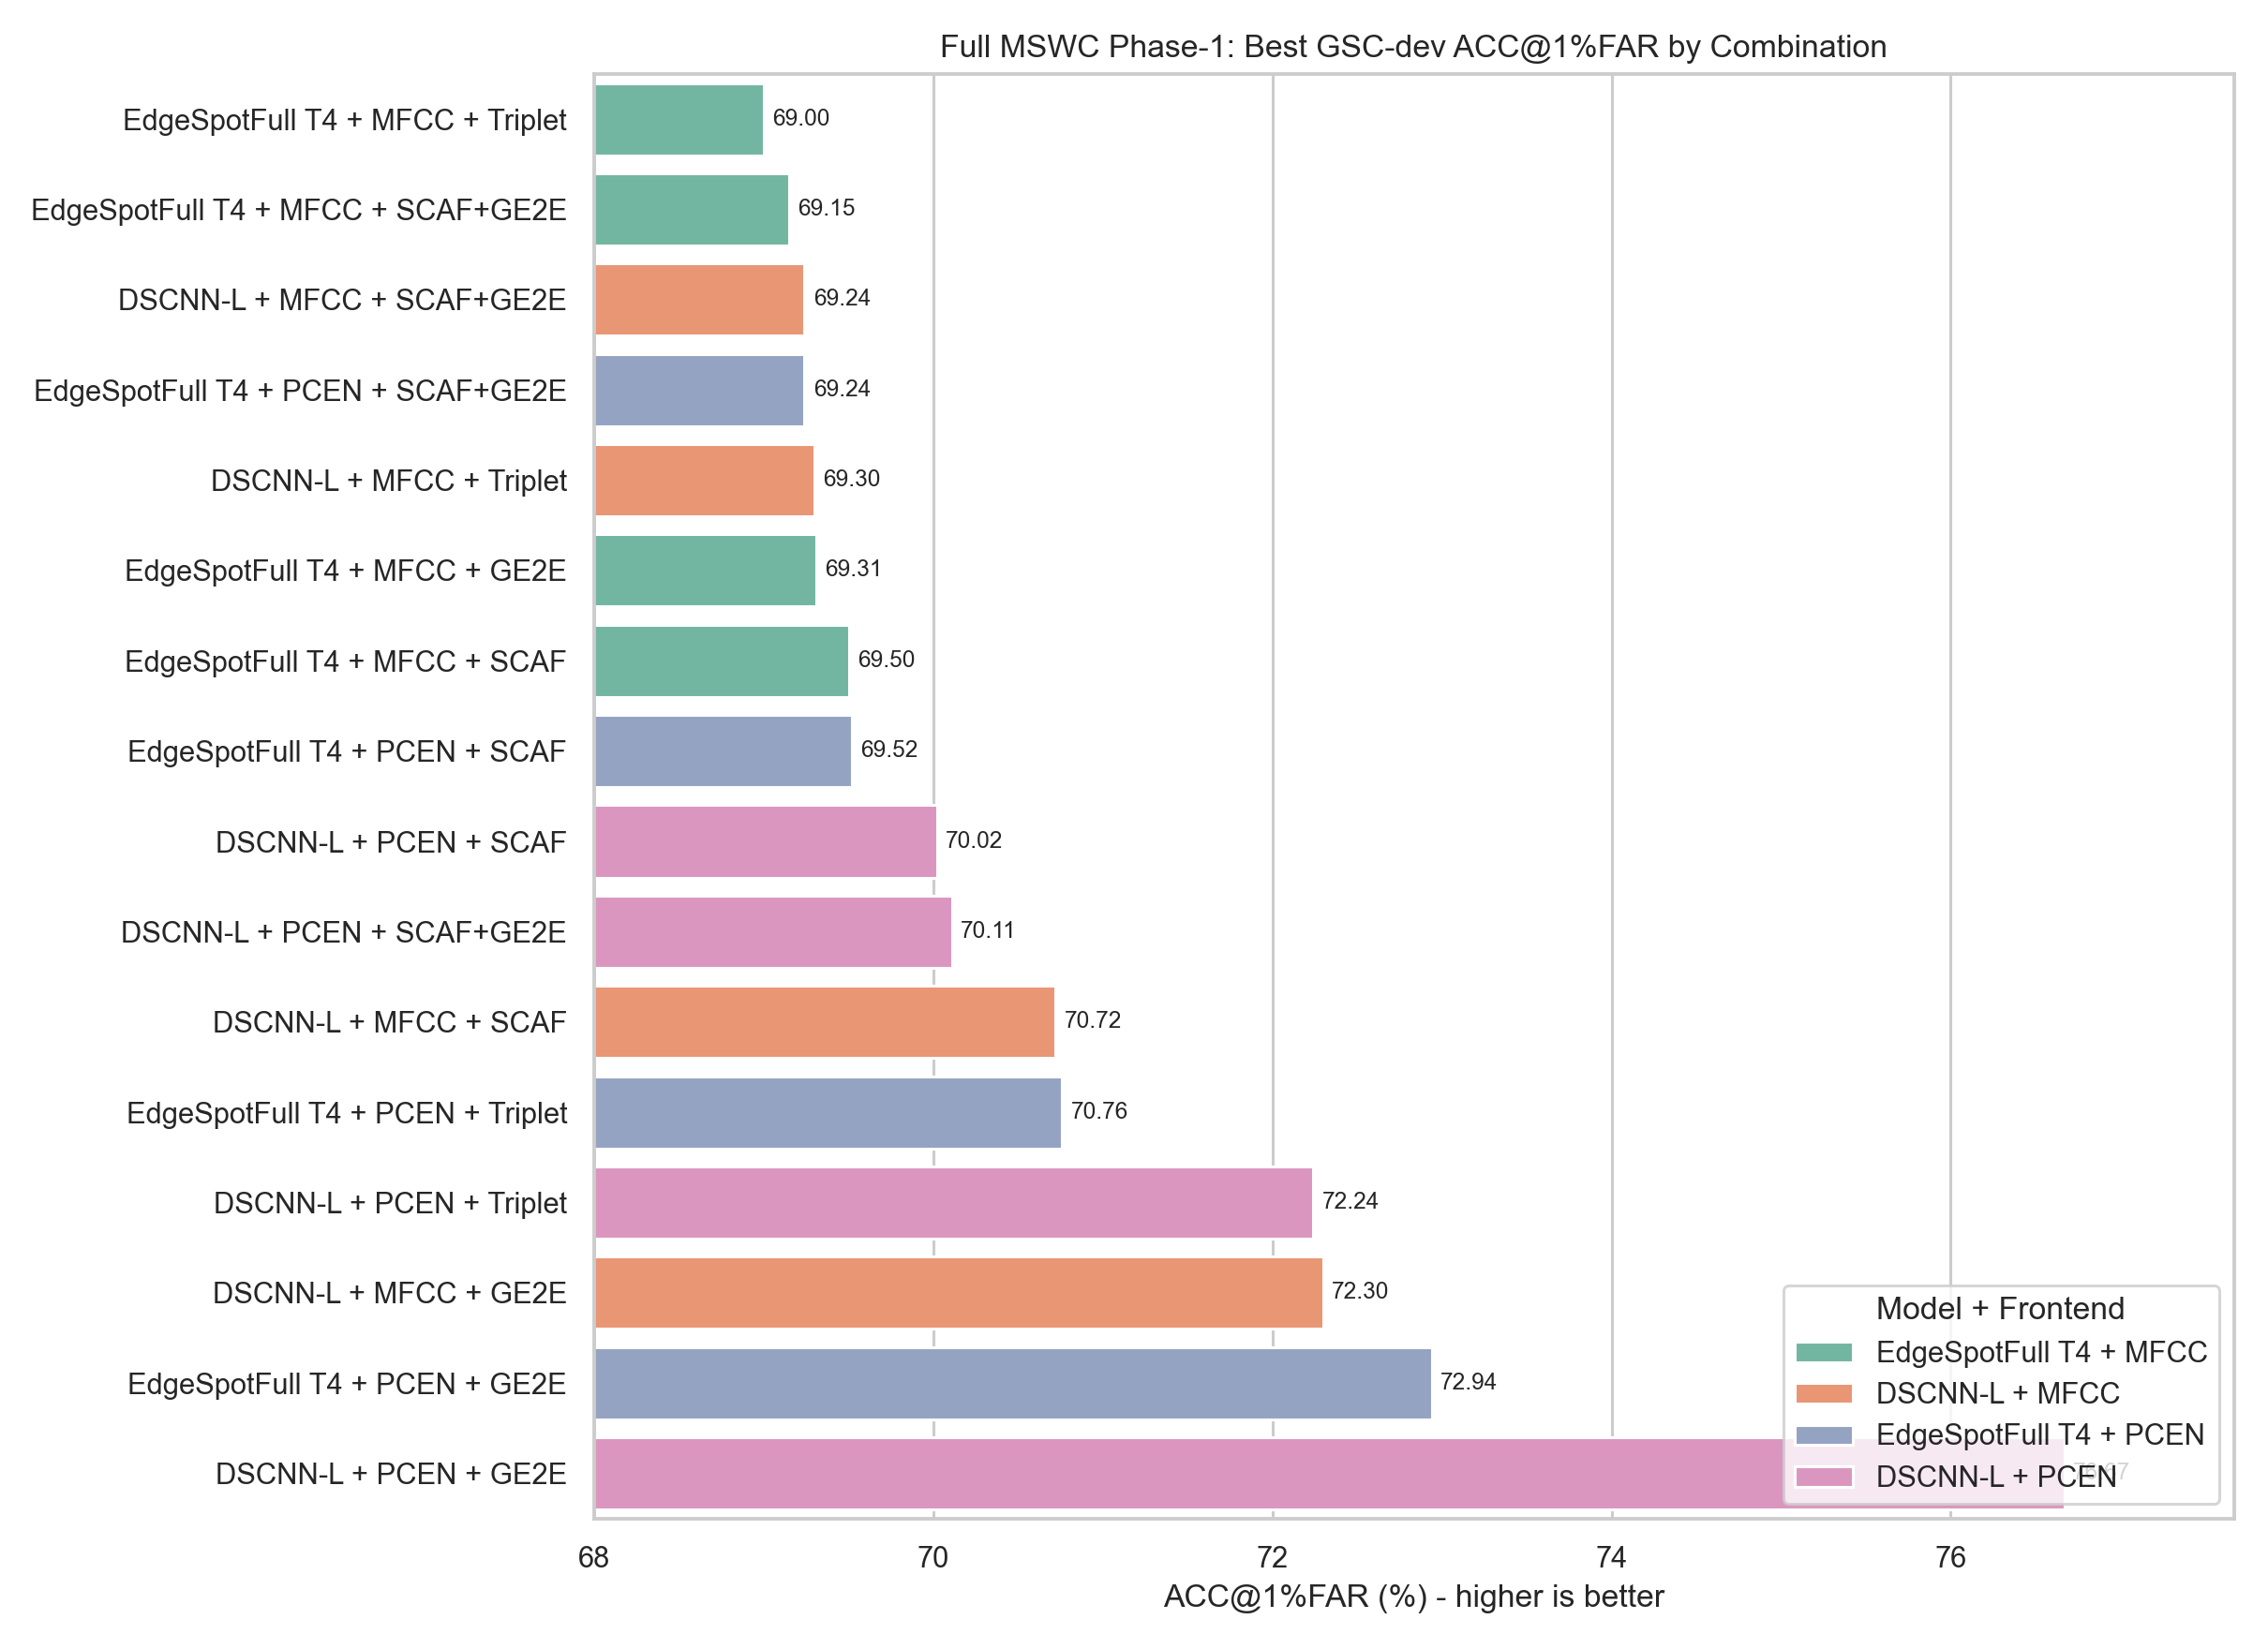
\includegraphics[width=0.96\linewidth]{res_ranked_bar.png}
\caption{Configurations ranked by GSC ACC@1\%FAR (phase-1 screen on full MSWC).
PCEN$+$GE2E pipelines lead; colour encodes backbone$\times$front-end.
\emph{Project-generated result figure.}}
\label{fig:ranked}
\end{figure}

\paragraph{Paired effect deltas.}
Isolating each axis (\Cref{tab:deltas}, \Cref{fig:deltas}) shows two robust wins.
PCEN improves every backbone --- most dramatically the edge encoder
($+9.22$ ACC, $+21.86$ F1) --- and GE2E consistently beats triplet. The
front-end therefore carries proportionally more of the representational burden
when the backbone is small.

\begin{table}[t]
\centering
\caption{Paired effect deltas (percentage points), full-vocabulary MSWC,
GSC test100 @ 1\% FAR. Positive favours the first option.}
\label{tab:deltas}
\small
\begin{tabular}{l r r r}
\toprule
\textbf{Contrast (others fixed)} & $\Delta\acc_{1\%}$ & $\Delta\auc$ & $\Delta$F1\\
\midrule
PCEN $-$ MFCC \;(DSCNN, GE2E)    & +5.26 & +5.96  & +9.25 \\
PCEN $-$ MFCC \;(Edge, GE2E)     & +9.22 & +21.93 & +21.86 \\
GE2E $-$ Triplet \;(DSCNN, PCEN) & +2.36 & +1.77  & +3.61 \\
DSCNN $-$ Edge \;(PCEN, GE2E)    & +2.36 & +5.19  & +7.07 \\
\bottomrule
\end{tabular}
\end{table}

\begin{figure}[t]
\centering
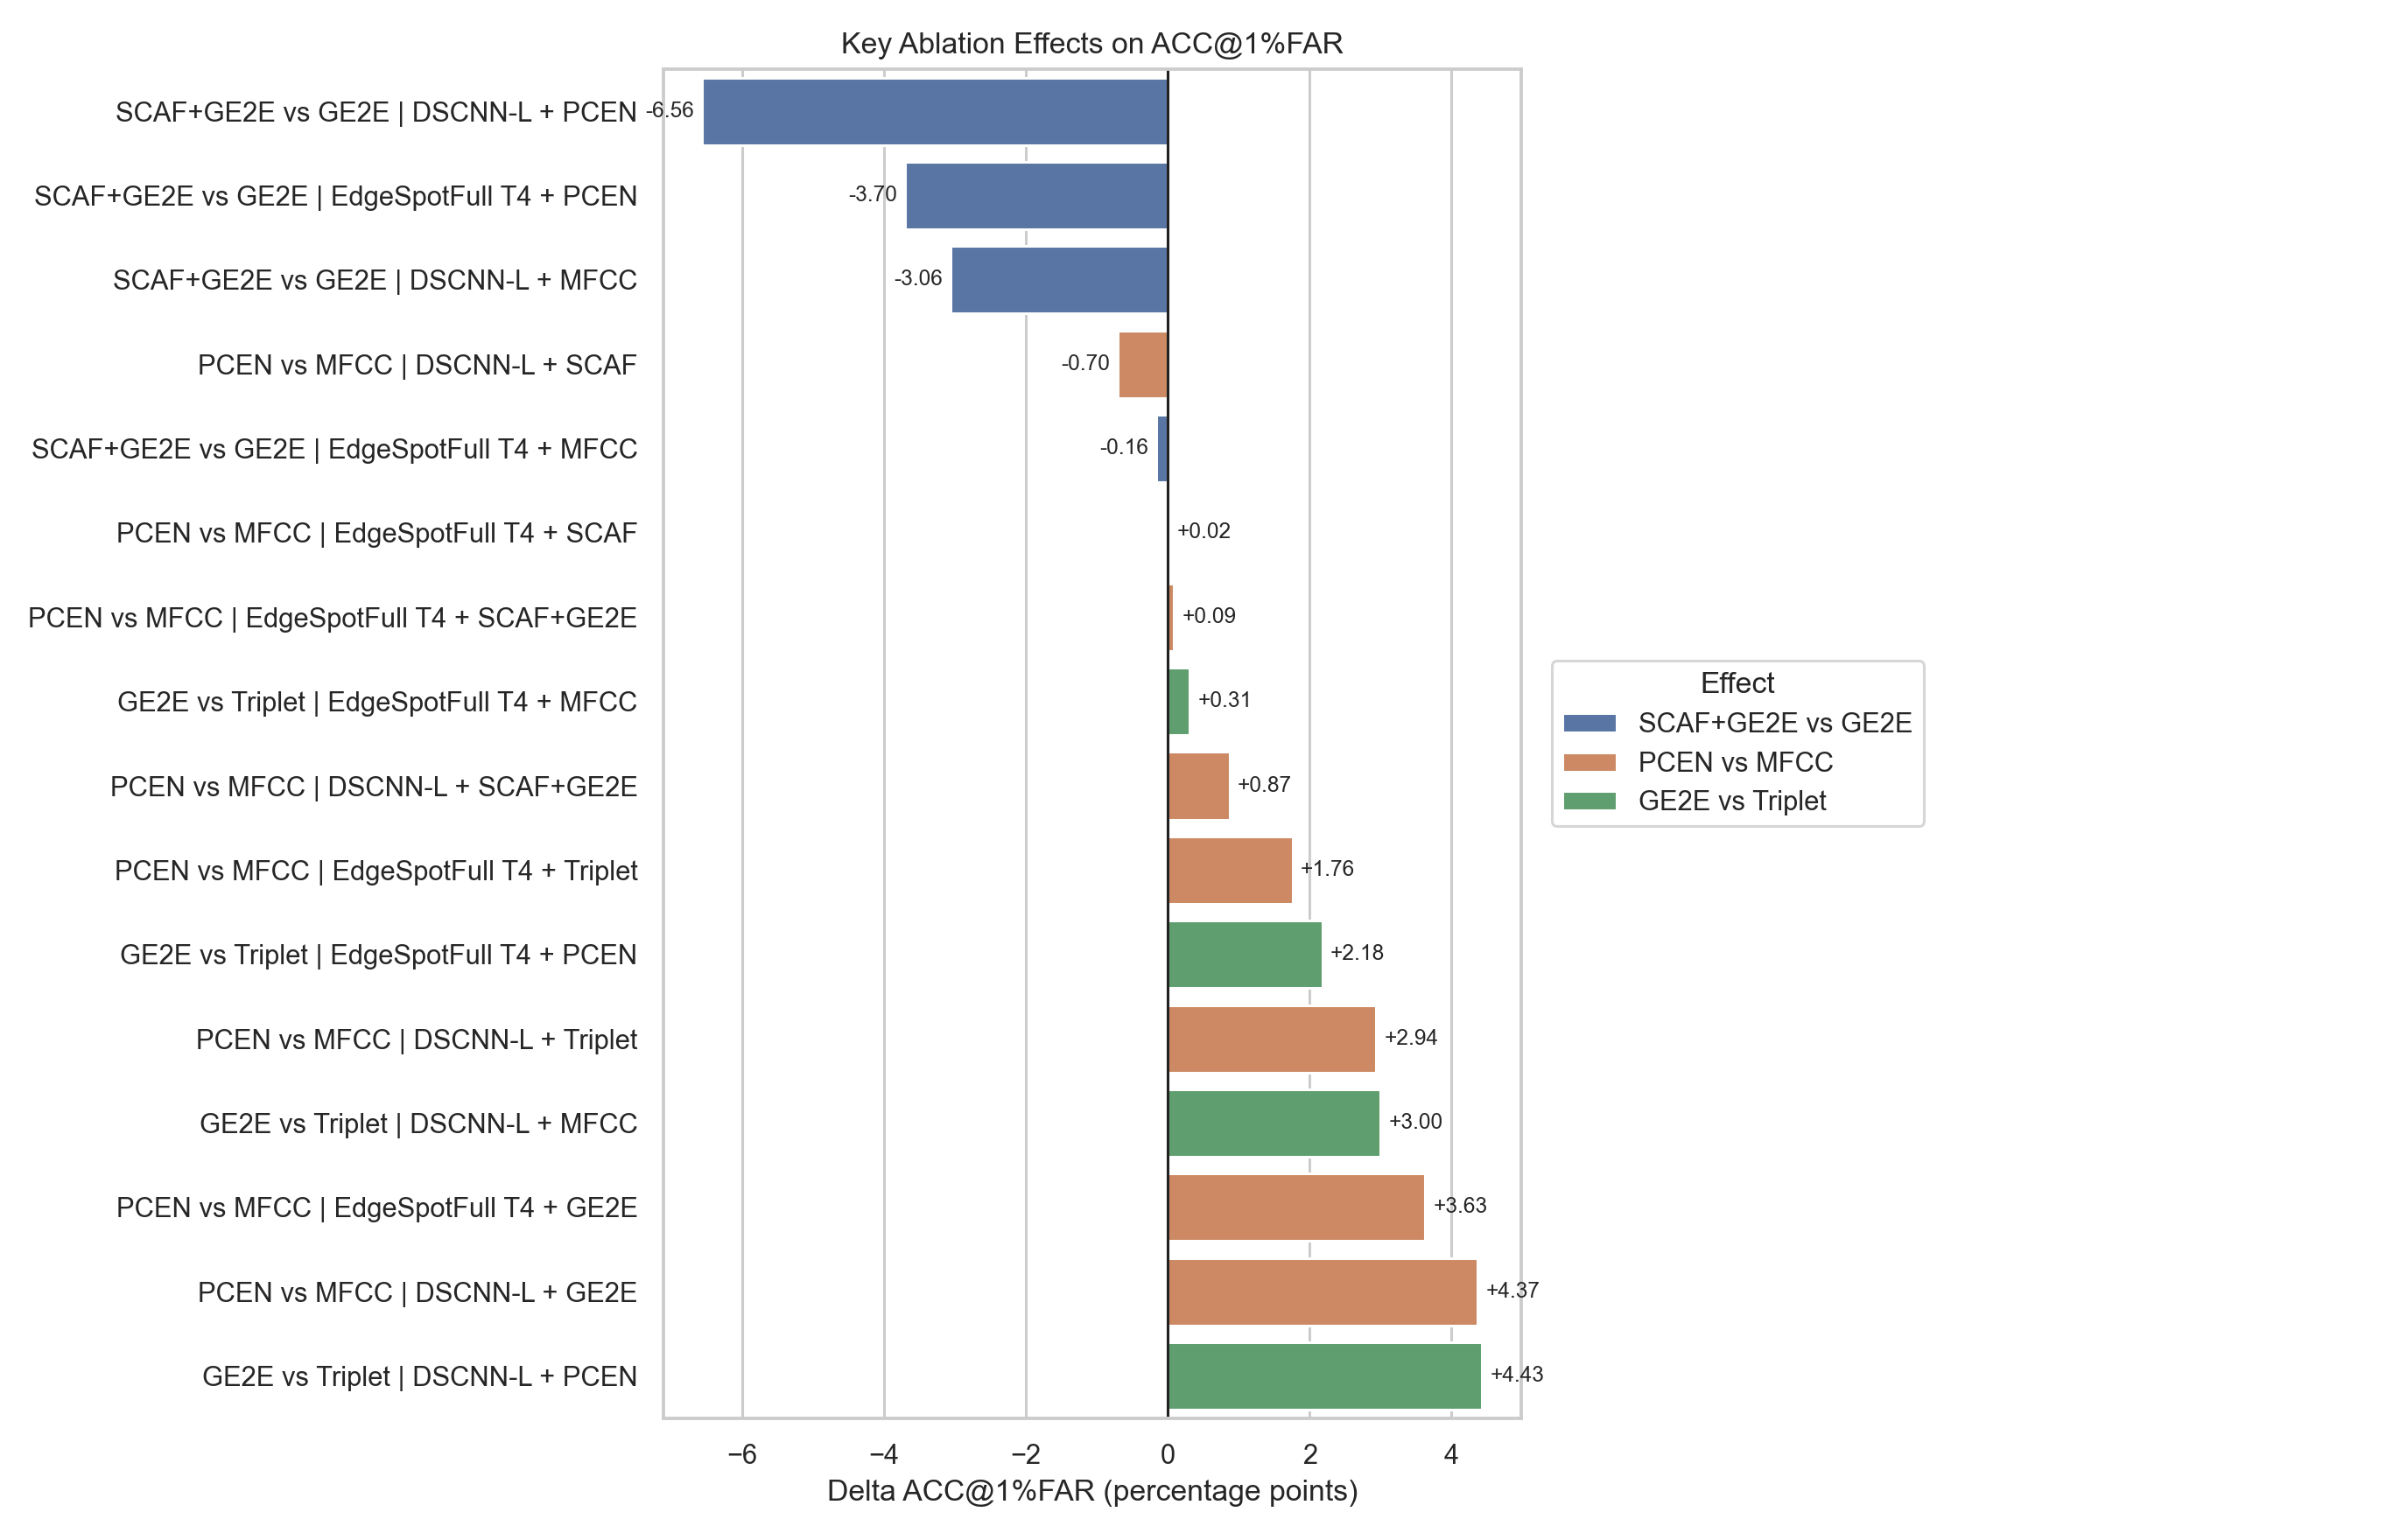
\includegraphics[width=0.92\linewidth]{res_effect_deltas.png}
\caption{Key paired effect deltas. PCEN and GE2E are the two consistent
improvements across backbones. \emph{Project-generated result figure.}}
\label{fig:deltas}
\end{figure}

\section{Q2: Scale --- saturation and the SCAF collapse}\label{sec:res-q2}

\paragraph{Accuracy saturates near 2\,M clips.}
\Cref{fig:saturation} and \Cref{tab:scale} sweep the per-word cap for the best
front-end/loss (PCEN$+$GE2E). There is a large jump between cap-50 and cap-220
($+3.55$ ACC for DSCNN, $+3.79$ for EdgeSpot at 5\% FAR) and a flat region from
cap-220 to cap-620 ($+0.33$/$-0.02$). Accuracy is effectively data-saturated at
$\sim$2\,M training clips: beyond this point, more clips of the same words yield
negligible cross-corpus gains.

\begin{figure}[t]
\centering
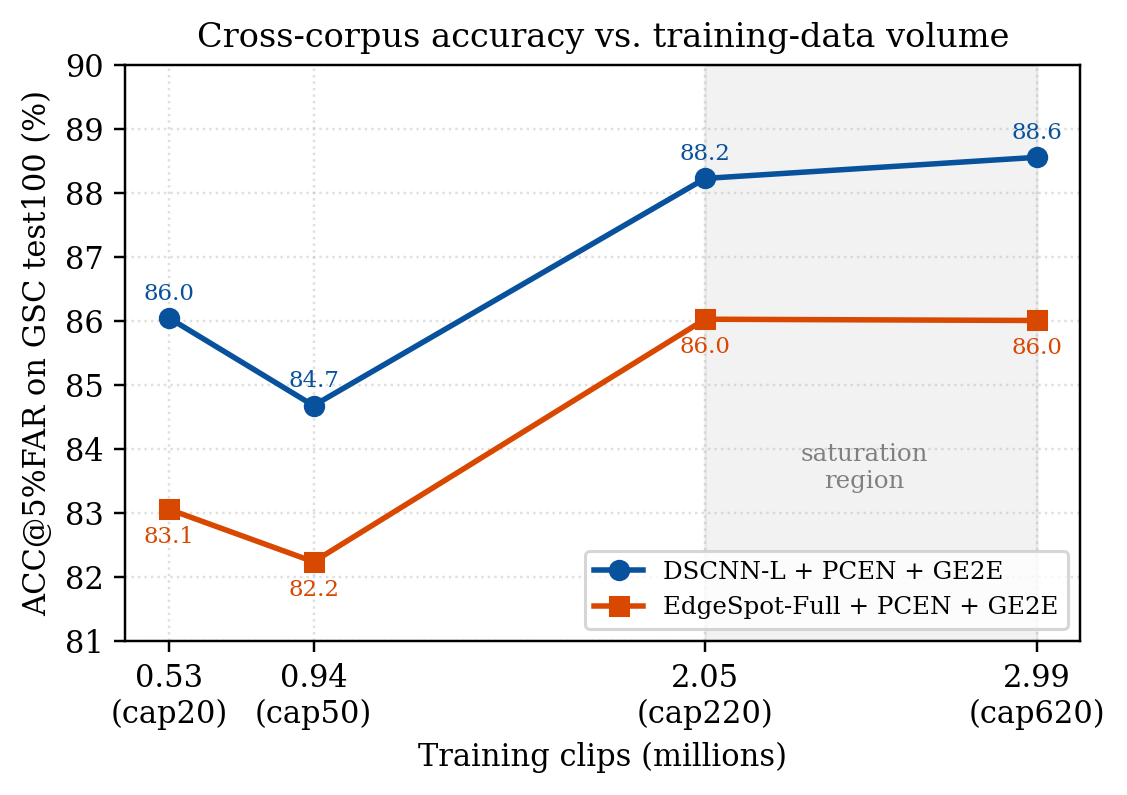
\includegraphics[width=0.80\linewidth]{fig_data_saturation.png}
\caption{Cross-corpus accuracy vs.\ training-data volume (per-word caps).
Performance saturates near $\sim$2\,M clips (shaded). \emph{Generated from
project results.}}
\label{fig:saturation}
\end{figure}

\begin{table}[t]
\centering
\caption{Data-scale sweep (PCEN$+$GE2E), GSC test100. ACC at 5\% FAR.}
\label{tab:scale}
\small
\begin{tabular}{l c r r r r}
\toprule
\textbf{Encoder} & \textbf{Cap} & \acc$_{5\%}$ & \auc & \eer & F1\\
\midrule
\multirow{4}{*}{DSCNN-L}
 & 20  & 86.05 & 91.57 & 16.25 & 75.90 \\
 & 50  & 84.68 & 90.45 & 17.42 & 74.34 \\
 & 220 & 88.23 & 93.87 & 12.78 & 80.67 \\
 & 620 & \best{88.56} & \best{94.04} & \best{12.53} & \best{81.02} \\
\midrule
\multirow{4}{*}{EdgeSpot}
 & 20  & 83.06 & 87.22 & 20.40 & 70.46 \\
 & 50  & 82.24 & 87.74 & 20.19 & 70.73 \\
 & 220 & \best{86.03} & 91.31 & 16.47 & 75.61 \\
 & 620 & 86.01 & \best{91.34} & 16.64 & 75.38 \\
\bottomrule
\end{tabular}
\end{table}

\paragraph{The SCAF collapse at 37k classes.}
The most striking result of the scale study is a qualitative failure. On the
31-class micro-set and the $\sim$500-class Top-500 split, SCAF and SCAF$+$GE2E are
excellent (AUC $\approx 95$; \Cref{sec:res-q4}). However, on the full
37,387-class vocabulary with the default SCAF weight of 1.0, training collapses
from epoch~2: validation AUC pins at 0.5000, the in-episode GE2E accuracy falls to
$\approx 0.033$ ($\approx 1/30$, i.e.\ chance), and the GSC metrics become
degenerate (AUC 50, F1 0, $\frr{=}100\%$, keyword ACC 9.09\%). The mechanism is a
gradient-magnitude imbalance: the sub-center ArcFace logit scale ($s{=}30$)
multiplied across $\sim$$3.7\times10^4$ classes produces a classification gradient
that dwarfs the centroid/cosine terms, driving all embeddings to a trivial
solution. The same hybrid does \emph{not} collapse under KD, where the SCAF weight
is $5\times10^{-5}$. The practical remedies we verify are: (i) reduce the SCAF
weight to $\sim$$5\times10^{-5}$, (ii) warm up the margin/scale, or (iii) drop the
classification term and use GE2E or KD. This is a cautionary result: angular-margin
classification losses that are state-of-the-art at $10^2$--$10^3$ classes do not
transfer naively to $10^4$-class word embedding.

\colabfig{Collapse curve for the \emph{full-vocabulary} SCAF$+$GE2E run (val AUC
pinned at 0.50 from epoch~2; in-episode accuracy $\sim$0.033). This specific run's
logs are \emph{not} in the local repo (only the Microset/Top500 logs are), so it
must be re-run on Colab --- see the runbook the assistant provided. Once you have
its \code{runs/} TensorBoard folder, plot it with the same
\code{make\_training\_curves.py} and save as \code{assets/scaf\_collapse.png}.
\textbf{Note: the healthy Microset training curve is already included as
\Cref{fig:traincurves}; this red box is only for the contrasting collapse run.}}

\section{Q3: Knowledge distillation trades teacher knowledge for data}\label{sec:res-q3}

\Cref{tab:kd} distills a frozen Wav2Vec\,2.0 teacher into the compact EdgeSpot
student. At cap-50, KD improves every metric over GE2E ($+3.60$ ACC@1\%FAR,
$-4.78$ EER, $+6.31$ F1) and, strikingly, KD at cap-50 matches GE2E at cap-220 ---
the same accuracy with roughly half the training clips. KD also saturates early
(cap-50$\to$cap-220 is essentially flat), indicating that the teacher injects most
of its useful inductive bias from limited data.

\begin{table}[t]
\centering
\caption{Knowledge distillation vs.\ GE2E (EdgeSpot student), GSC test100.}
\label{tab:kd}
\small
\begin{tabular}{l l r r r r}
\toprule
\textbf{Cap} & \textbf{Loss} & \acc$_{1\%}$ & \acc$_{5\%}$ & \eer & F1\\
\midrule
50  & GE2E & 77.14 & 82.24 & 20.19 & 70.73 \\
\rowcolor{blue!7}
50  & KD   & \best{80.74} & \best{85.82} & \best{15.41} & \best{77.04} \\
220 & GE2E & --    & 86.03 & 16.47 & 75.61 \\
220 & KD   & 80.82 & 85.90 & 15.36 & 77.10 \\
\bottomrule
\end{tabular}
\end{table}

\section{Q4: Best deployable systems}\label{sec:res-q4}

\Cref{tab:final} consolidates the strongest configurations per data regime, and
\Cref{fig:detcurve,fig:heatmap} visualize the headline operating point. Three
points stand out:
\begin{itemize}[leftmargin=1.3em,itemsep=2pt]
\item \textbf{Best overall:} DSCNN-L$+$PCEN$+$GE2E (cap-620) reaches
\best{$86.36\pm1.29$} ACC@1\%FAR and $89.93\pm0.65$ at 5\% FAR, with AUC 95.21,
EER 11.32, F1 82.73, keyword ACC 92.92\%.
\item \textbf{Best compact:} EdgeSpot-Full$+$PCEN$+$GE2E (cap-620) reaches
$82.87\pm1.22$ ACC@1\%FAR at 0.131\,M parameters --- within $\sim$3.5 points of the
best system at one third the size, and on par with the EdgeSpot-4 literature
reference ($\sim$82\% ACC@1\%FAR, $\sim$128k params).
\item \textbf{Best small-vocabulary:} on the reduced Top-500 split, the
EdgeSpot$+$PCEN$+$SCAF$+$GE2E hybrid is the strongest compact model
($85.62\pm1.04$ ACC@1\%FAR, AUC 95.34), confirming that the hybrid is excellent
\emph{when the class count is small enough not to trigger the collapse}.
\end{itemize}

\begin{table}[t]
\centering
\caption{Consolidated best systems across data regimes (GSC test100,
EdgeSpot-exact 10-shot, 100 runs). ``coll.''$=$ degenerate collapse.}
\label{tab:final}
\small
\setlength{\tabcolsep}{4pt}
\begin{tabular}{l l l c r r r r r r}
\toprule
\textbf{Regime} & \textbf{Encoder} & \textbf{Loss} & \textbf{Params} &
\acc$_{1\%}$ & \acc$_{5\%}$ & \auc & \eer & F1 & KW\\
\midrule
Micro (31)    & EdgeSpot & SCAF+GE2E      & 0.131M & 84.61 & 86.12 & 95.61 & 11.54 & 82.41 & 77.66 \\
Top-500       & EdgeSpot & SCAF+GE2E\,ep13& 0.131M & 85.62 & 88.79 & 95.34 & 11.51 & 82.45 & 90.44 \\
Top-500       & DSCNN-L  & GE2E           & 0.413M & 81.55 & 86.56 & 93.17 & 14.00 & 78.97 & 88.62 \\
Full cap20    & DSCNN-L  & GE2E           & 0.413M & 82.10 & 86.05 & 91.57 & 16.25 & 75.90 & 88.90 \\
Full cap220   & DSCNN-L  & GE2E           & 0.413M & --    & 88.23 & 93.87 & 12.78 & 80.67 & 89.82 \\
\rowcolor{blue!7}
Full cap620   & DSCNN-L  & GE2E\,ep300    & 0.413M & \best{86.36} & \best{89.93} & \best{95.21} & \best{11.32} & \best{82.73} & \best{92.92} \\
Full cap620   & EdgeSpot & GE2E\,ep300    & 0.131M & 82.87 & 86.76 & 92.41 & 14.82 & 77.85 & 87.29 \\
Full cap50    & EdgeSpot & KD             & 0.131M & 80.74 & 85.82 & 91.19 & 15.41 & 77.04 & 87.95 \\
Full cap220   & EdgeSpot & SCAF+GE2E      & 0.131M & coll. & coll. & 50.00 & 50.00 & coll. & 9.09 \\
\bottomrule
\end{tabular}
\end{table}

\begin{figure}[t]
\centering
\begin{subfigure}{0.49\linewidth}
  \centering
  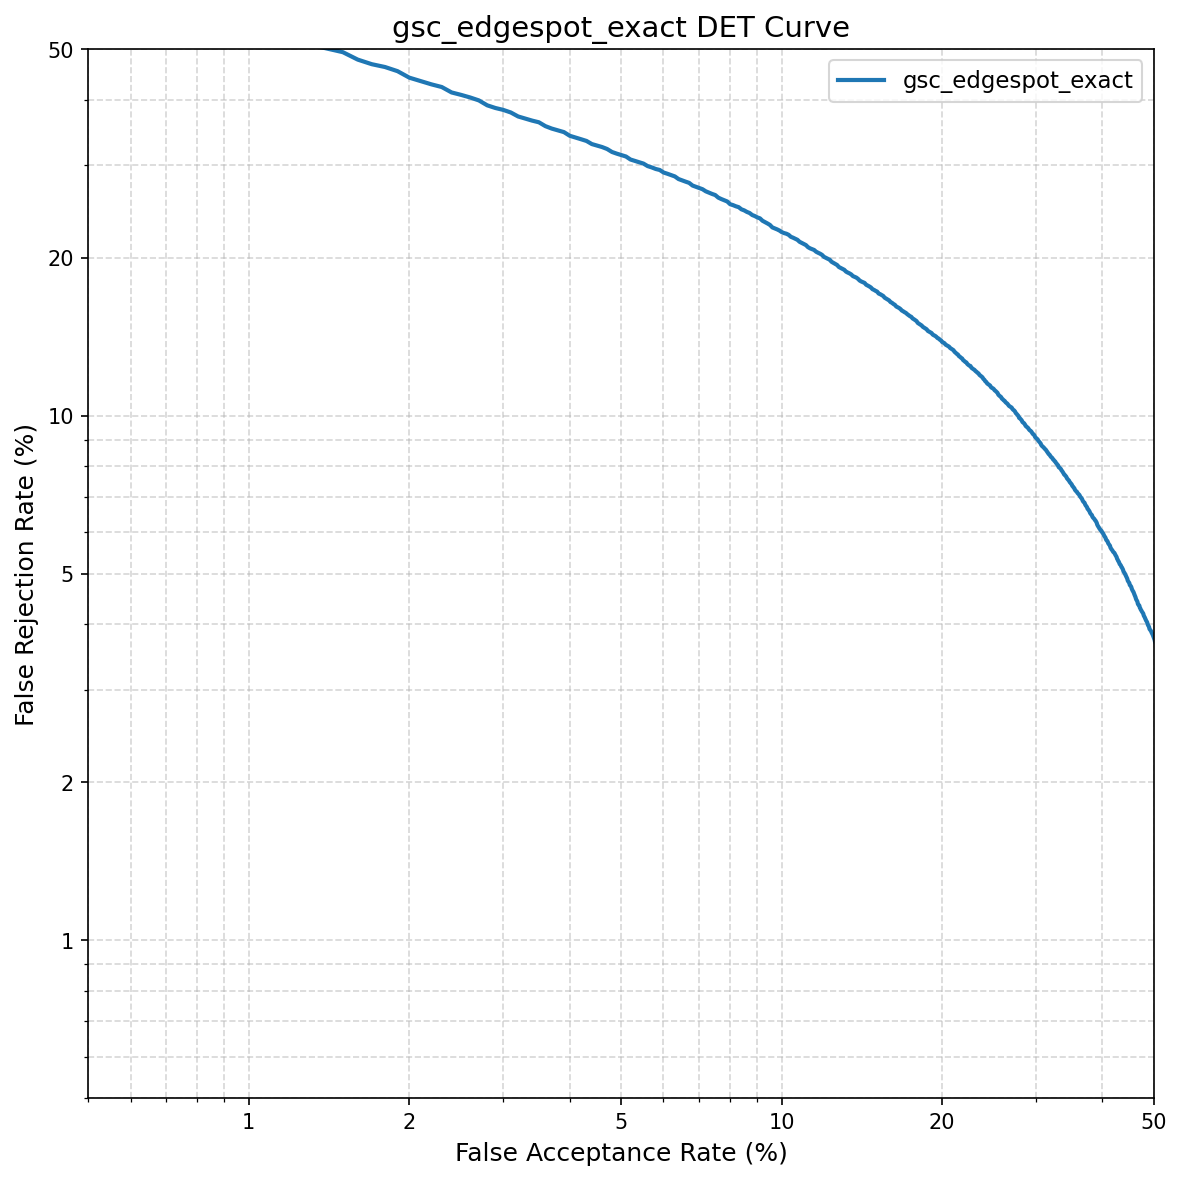
\includegraphics[width=\linewidth]{res_det_dscnn.png}
  \caption{DET curve (DSCNN-L$+$PCEN$+$GE2E).}
  \label{fig:detcurve}
\end{subfigure}\hfill
\begin{subfigure}{0.49\linewidth}
  \centering
  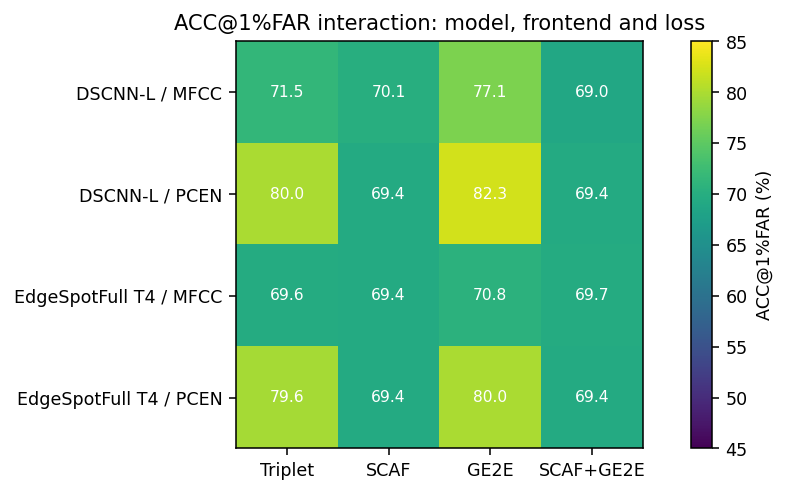
\includegraphics[width=\linewidth]{res_cap620_heatmap.png}
  \caption{ACC@1\%FAR heat map (cap-620).}
  \label{fig:heatmap}
\end{subfigure}
\caption{Headline operating-point views. (a) Detection-error-tradeoff curve of the
best overall system; (b) accuracy heat map over the cap-620 configurations.
\emph{Project-generated result figures.}}
\label{fig:res-q4}
\end{figure}

\section{Inference on long audio}\label{sec:res-inference}
\reviewnote{New section, the analogue of the sample thesis's ``Inference'' results.
\Cref{fig:longinfer} is produced by actually running the trained model on a real
multi-word recording.}

To verify that the system behaves end-to-end --- not only on isolated test clips ---
we enroll prototypes for 17 keywords (10 shots each from GSC) and run
nearest-prototype inference over a real, continuously spoken multi-word recording.
\Cref{fig:longinfer} overlays the predicted keyword and its prototype distance on
the waveform for the first 16 spoken segments. The model correctly identifies
$15/16$ segments ($\approx$94\%); the single error (``sheila'', a long, rare name)
also has the largest prototype distance, exactly the signal the open-set threshold
uses to flag low-confidence detections.

\begin{figure}[t]
\centering
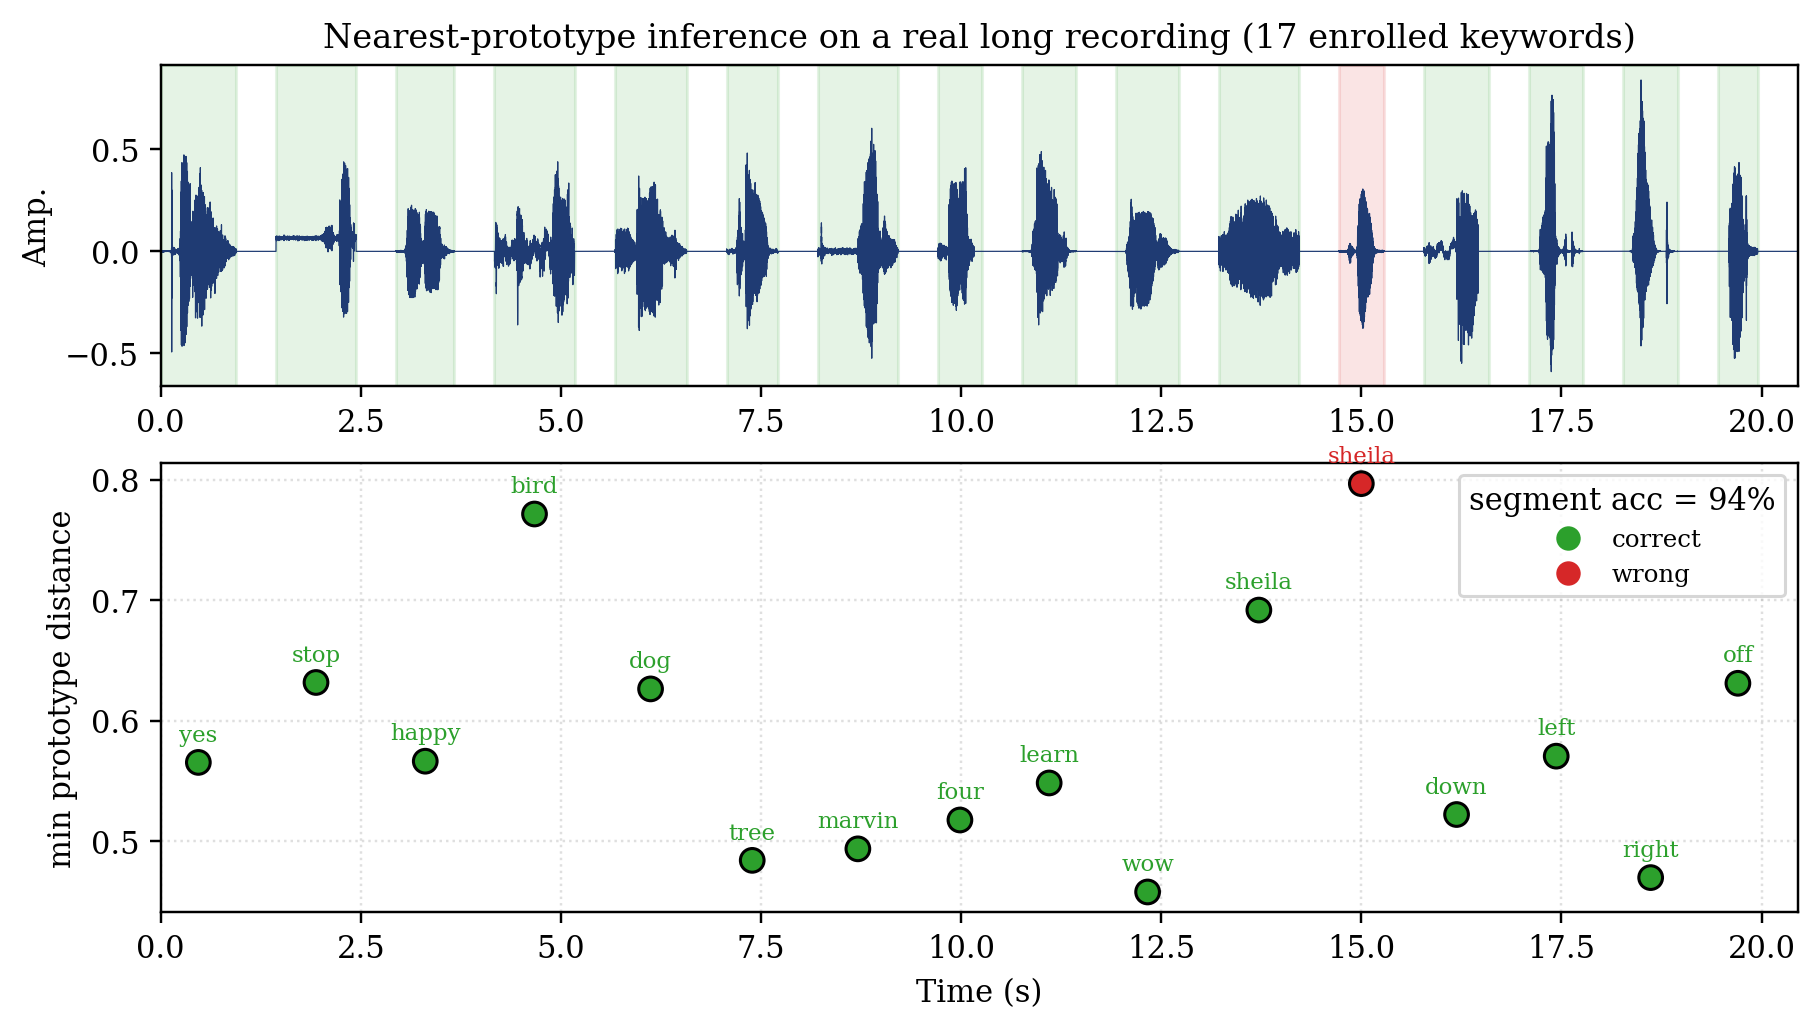
\includegraphics[width=0.98\linewidth]{fig_long_inference.png}
\caption{\NEW{Nearest-prototype inference on a real long recording. Top: waveform
with per-segment correct (green) / wrong (red) shading. Bottom: minimum prototype
distance and predicted keyword per segment. Generated from the local checkpoint
with \code{make\_inference\_figures.py}.}}
\label{fig:longinfer}
\end{figure}

\begin{figure}[t]
\centering
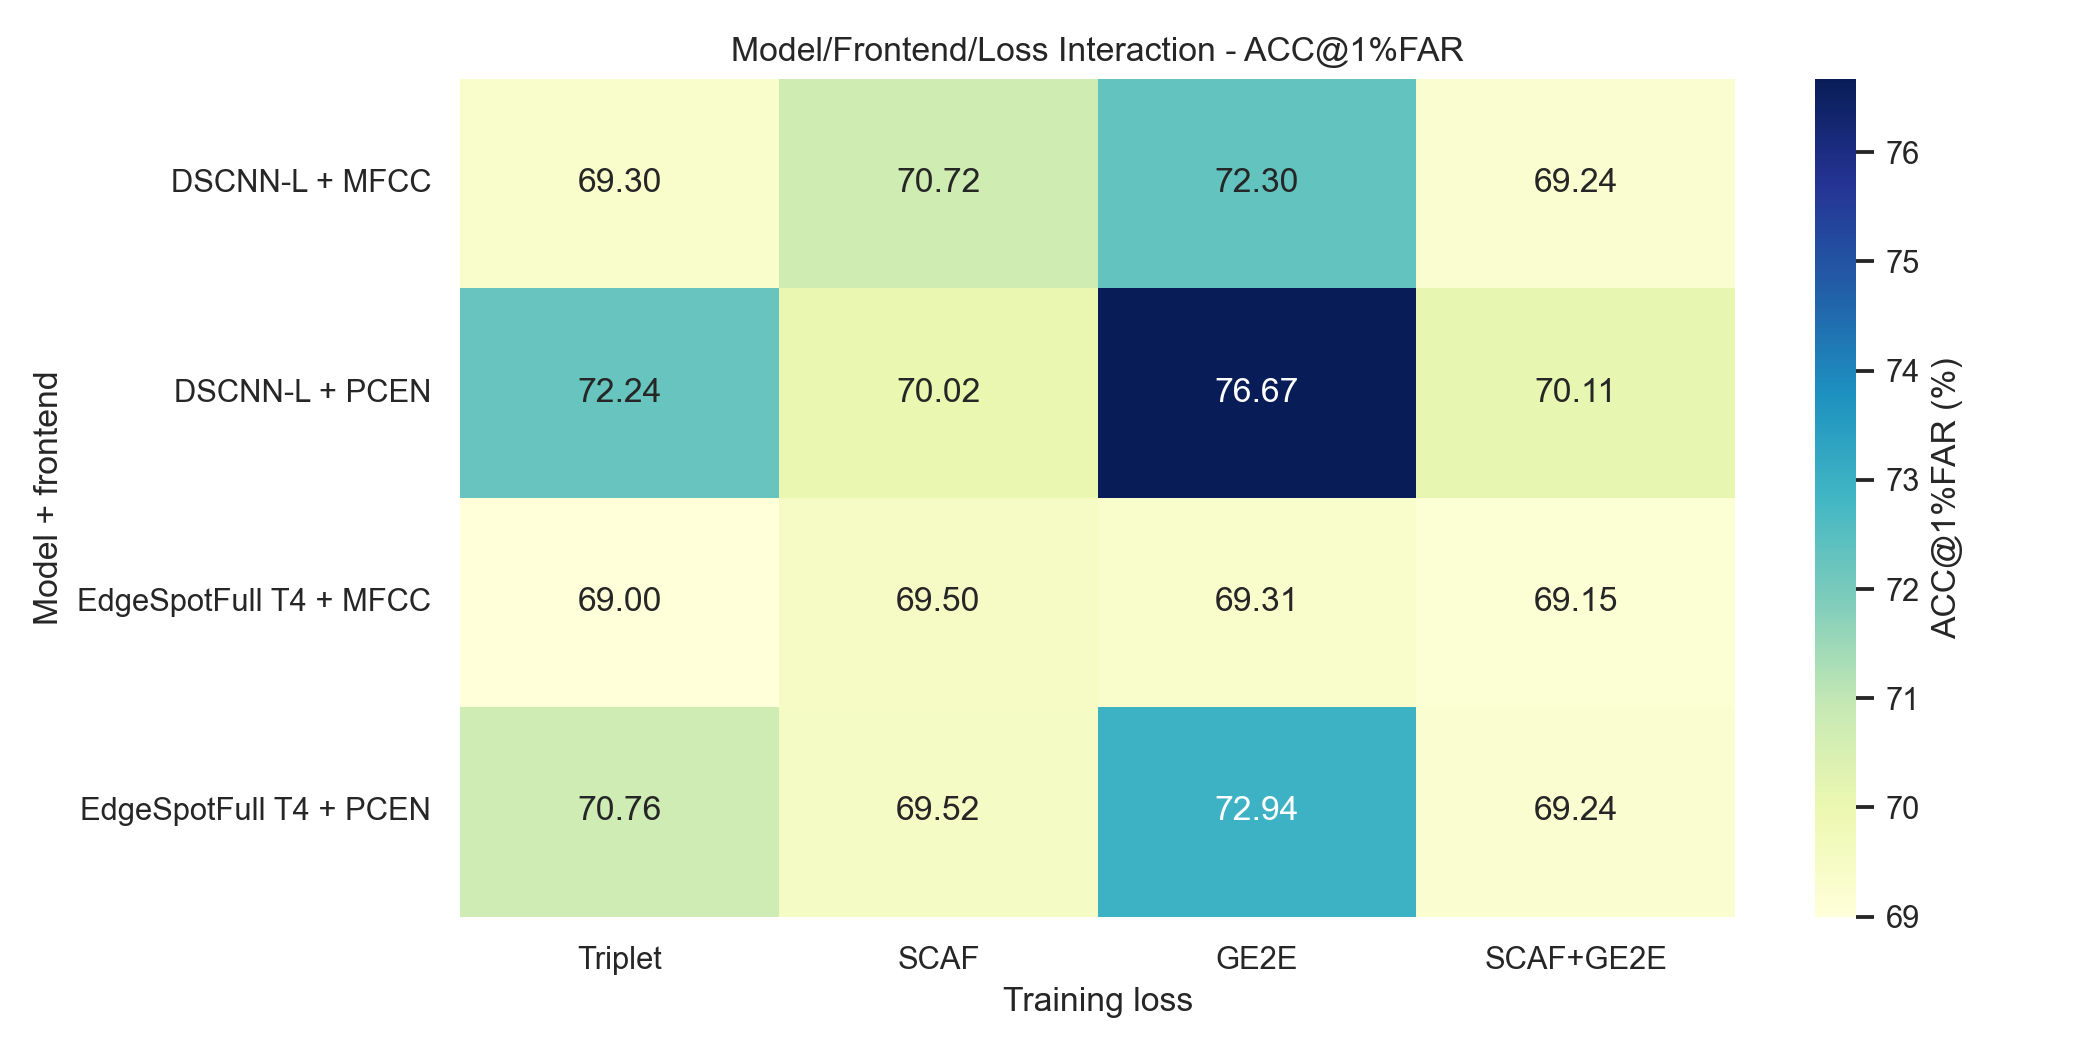
\includegraphics[width=0.82\linewidth]{res_interaction_heatmap.png}
\caption{\NEW{Front-end $\times$ loss interaction (ACC@1\%FAR). The PCEN$+$GE2E cell
dominates; classification-only cells degrade at full vocabulary scale.}}
\label{fig:interaction}
\end{figure}

\paragraph{Reproducibility note on data regimes.}
Within full-vocabulary results, three cap-620 runs use different episode budgets
(a 40-epoch fixed screen, a 1000-episode saturation run, and a 300-episode
composite-selection development run). They must not be conflated; each table row
is drawn from a single consistent run, with the budget stated where it matters.

%==============================================================================
\chapter{Conclusion}\label{ch:conclusion}
\reviewnote{This chapter is new ($\sim$2 pages as requested): current status, what
is good, what is weak, and future work.}

\section{Current status}\label{sec:status}

This thesis set out to build a keyword-spotting system that escapes the two
structural limits of classical wake-word engines --- a frozen vocabulary and the
inability to abstain --- and to understand, rather than merely report, what makes
such a system work as the training vocabulary grows. We delivered a complete,
reproducible, dependency-light pipeline: two compact encoders (DSCNN-L at
$\approx$0.41\,M and EdgeSpot-Full at $\approx$0.13\,M parameters), three feature
front-ends, four metric-learning objectives, four open-set rejection heads, a
CPU streaming engine, and an offline web demonstrator. Every system is trained on
MSWC English and evaluated cross-corpus on GSC v2 under a single strict
EdgeSpot-exact 10-shot protocol with 100 randomized runs, so the numbers compare
fairly.

The headline outcome is that few-shot open-set KWS is viable and even strong at
true vocabulary scale: training once on $37{,}387$ words, the best configuration
(DSCNN-L $+$ PCEN $+$ GE2E) reaches $86.36\%$ open-set accuracy at a strict
$1\%$ false-accept rate and $95.21$ AUC on a corpus it was never trained on, while
a three-times-smaller edge model stays within a few points. A user can define an
arbitrary keyword set from ten examples per word, with no retraining, and the
system can decline to answer on unknown speech and silence.

\section{What is good, what is weak}\label{sec:goodbad}

\paragraph{What works.} Three findings are robust and transferable. (1) The
trainable PCEN front-end is the most reliable single improvement, and it helps the
smaller encoder most --- a useful lever precisely where parameter budget is
tightest. (2) The centroid GE2E objective, which optimizes the same enroll-then-match
computation used at deployment, consistently beats both triplet and
classification objectives for open-set generalization. (3) A frozen Wav2Vec\,2.0
teacher distilled with a simple cosine loss lets the compact model reach
GE2E-level accuracy with roughly half the data, which matters when data or compute
are limited.

\paragraph{What is weak / what we learned the hard way.} The clearest negative
result is the collapse of the sub-center ArcFace (SCAF) classification objective at
$10^4$-class scale: a loss that is excellent on tens to hundreds of classes drives
the embedding to a trivial solution on tens of thousands of classes unless its
weight is cut by four orders of magnitude. This is an important cautionary lesson
for anyone scaling angular-margin losses to large label spaces. Two further
limitations bound the present claims. First, the ACC@FAR/FRR@FAR operating points
are read from the evaluation ROC (an oracle threshold) rather than transferred
from an independent calibration split; we mitigate this by always co-reporting
threshold-free AUC/EER/F1, but a calibrated, deployment-time threshold study is
still owed. Second, enrollment is fixed at $k{=}10$ shots and the streaming
latency figures are design budgets, not measured field benchmarks; there is also
no quantitative denoising ablation.

\section{Future work}\label{sec:future}

Four directions follow directly from the limitations above.
(1) \emph{$k$-shot sensitivity:} sweep $k\in\{1,3,5,10\}$ to chart the
accuracy-vs-enrollment-effort curve, which is the metric end users actually feel.
(2) \emph{Calibrated thresholds:} learn or transfer the open-set threshold from a
held-out split and report deployment-realistic ACC@FAR, closing the oracle gap.
(3) \emph{On-device benchmark:} measure end-to-end latency, false-alarms-per-hour
and miss-rate on target hardware, and an SNR-sweep denoising ablation, to validate
the design budgets.
(4) \emph{Stabilizing classification at scale:} margin/scale warm-up, curriculum,
or sub-center pruning to recover the discriminative power of angular-margin losses
without the collapse --- potentially combining SCAF's tight clusters with GE2E's
deployment-matched objective at full vocabulary.

In summary, the thesis demonstrates a deployable, retraining-free, open-set
keyword spotter and, just as importantly, a clear empirical map of which design
choices help, where they saturate, and where they fail as the problem scales.

%==============================================================================
\begin{thebibliography}{99}
\footnotesize

\bibitem{zhang2017hello} Y.~Zhang, N.~Suda, L.~Lai, and V.~Chandra,
``Hello edge: Keyword spotting on microcontrollers,'' \emph{arXiv:1711.07128}, 2017.
\bibitem{kim2021bcresnet} B.~Kim, S.~Chang, J.~Lee, and D.~Sung,
``Broadcasted residual learning for efficient keyword spotting,'' \emph{Interspeech}, 2021.
\bibitem{snell2017prototypical} J.~Snell, K.~Swersky, and R.~Zemel,
``Prototypical networks for few-shot learning,'' \emph{NeurIPS}, 2017.
\bibitem{schroff2015facenet} F.~Schroff, D.~Kalenichenko, and J.~Philbin,
``FaceNet: A unified embedding for face recognition and clustering,'' \emph{CVPR}, 2015.
\bibitem{wan2018ge2e} L.~Wan, Q.~Wang, A.~Papir, and I.~L.~Moreno,
``Generalized end-to-end loss for speaker verification,'' \emph{ICASSP}, 2018.
\bibitem{deng2019arcface} J.~Deng, J.~Guo, N.~Xue, and S.~Zafeiriou,
``ArcFace: Additive angular margin loss for deep face recognition,'' \emph{CVPR}, 2019.
\bibitem{deng2020subcenter} J.~Deng, J.~Guo, T.~Liu, M.~Gong, and S.~Zafeiriou,
``Sub-center ArcFace: Boosting face recognition by large-scale noisy web faces,'' \emph{ECCV}, 2020.
\bibitem{bendale2016openmax} A.~Bendale and T.~E.~Boult,
``Towards open set deep networks,'' \emph{CVPR}, 2016.
\bibitem{liu2020energy} W.~Liu, X.~Wang, J.~Owens, and Y.~Li,
``Energy-based out-of-distribution detection,'' \emph{NeurIPS}, 2020.
\bibitem{wang2017trainable} Y.~Wang, P.~Getreuer, T.~Hughes, R.~F.~Lyon, and R.~A.~Saurous,
``Trainable frontend for robust and far-field keyword spotting,'' \emph{ICASSP}, 2017.
\bibitem{baevski2020wav2vec} A.~Baevski, H.~Zhou, A.~Mohamed, and M.~Auli,
``wav2vec 2.0: A framework for self-supervised learning of speech representations,'' \emph{NeurIPS}, 2020.
\bibitem{mazumder2021mswc} M.~Mazumder \emph{et al.},
``Multilingual Spoken Words Corpus,'' \emph{NeurIPS Datasets and Benchmarks}, 2021.
\bibitem{warden2018speech} P.~Warden,
``Speech Commands: A dataset for limited-vocabulary speech recognition,'' \emph{arXiv:1804.03209}, 2018.

\end{thebibliography}

\end{document}
